
\section{Differential geometry on general relativity}

\subsection{Introduction}
%
\theme{Source:} this section summarizes \cite{bertschinger:1999}.

\theme{Requirement:} general relativity (GR) requires familiarity with the geometrical properties of curved spacetime.

\theme{GR essential ideas:} a curved, four-dimensional pseudo-Riemannian manifold models spacetime. At every event (spacetime point), general relativity physics is locally special relativity physics. Mass (as mass and momentum flux) curves spacetime as described by Einstein's field equations.

\theme{Events:} Points in spacetime.

\theme{Covariant principle:} the laws of physics must be expressed in a form that is valid independently of any coordinate system used to label events.

\theme{Geometric description} of GR is better suited to develop physical understanding and thus used for theoretical work. Components and coordinate systems are useful for calculations \emph{once a coordinate system is chosen} .

\theme{Conventions and notation:} assume units where \lingo{speed of light of vacuum} is unity, $\klight = 1$. \emph{Greek} indices ranging from 0 to 3 will represent tensorial components. \lingo{Coordinate-free notation}, \lingo{abstract index notation}, and \lingo{Einstein's summation convention} are used. Vectors will be decorated with an arrow, $\vec v$, while covectors with a tilde, $\cov p$. Events will be denoted with calligraphic fonts, $\event P$. Event positions on spacetime by $\vec\pos\vat{\event P}$, or shortened to $\vec\pos$. Event coordinates $\tvec\pos\mu\vat{\event P}$, or shortened to $\tvec\pos\mu$. The flat spacetime metric (Minkowski metric) components are $\tvecfmet\mu\nu = \diag\tuple{-1,+1,+1,+1}$.


\subsection{Vectors and covectors}
%
\theme{GR math:} differential geometry: the math of smoothly curved (hyper-)surfaces: differentiable manifolds.

\theme{Geometry} models physics, thus keep in mind the geometrical interpretation of physical quantities.

\theme{Plan:} introduction of geometric objects in a coordinate-free manner. Then, coordinates to simplify calculations.

\theme{Main geometric objects:} scalars, vectors, covectors, and tensors.


\subsubsection{Vectors}
%
\theme{Vector:} a quantity with a magnitude and a direction. Vectors form a linear space (linear algebra, \aka\ vector space); \ie, it's possible to add vectors and multiply them by scalars. Addition is closed.

Scalars and vectors are \lingo{invariant} under coordinate transformations; vector \emph{components} are not.

\theme{Events:} denote events in spacetime by $\event P$. This notation refers to a point in spacetime \emph{not} to a vector. So there's no need to think of vectors going from an origin to a point.

\theme{Separation:} as long as space is smooth (as assumed by considering a differentiable manifold), it's possible to define the separation (vector) $d\vec\sep$ between two infinitesimally close events, say $\event P,\event Q$. The set of all $d\vec\sep_\event{P}$ defines a tangent space at $\event P$. 

\theme{Vector field:} by assigning a tangent vector to \emph{every} event, we define a vector field at $\event P$.


\subsubsection{Covectors and dual vector space}
%
\theme{Covector:} defined as a linear scalar function of a vector; \ie, a covector takes a vector as input and outputs a scalar. 

Consider a covector $\cov p$, a linear space $\lspace V$, and a vector $\vec v\in\lspace V$. Then, 
%
\begin{equation*}
  \fdef{\cov p}{\lspace V}{\rspace}\suchthat\fmap{\vec v}{\rspace}\,.
\end{equation*}

\theme{Scalar product:} the action of $\cov p$ on $\vec v$, $\cov p\vat{\vec v}$, denoted with angle brackets:
%
\begin{equation}\label{eq:scalarproductcovectoronvector}
  \cov p\vat{\vec v} \defas \sprod{\cov p}{\vec v}\,.
\end{equation}

\theme{Notation:} use a right arrow $\vslot$ to denote a vector argument of a function, a tilde $\cslot$ for a covector argument, and a check mark $\fslot$ for a taken argument.

\theme{Scalar product operator:} binary operator taking a covector and a vector to return a scalar, $s\in\rspace$
%
\begin{equation*}
  \fdef{\sprod\cslot\vslot}{\dlspace V\setprod\lspace V}{\rspace}\suchthat\fmap{\tuple{\cov p, \vec v}}{s}\,,
\end{equation*}
%
\theme{Note:} as defined, the scalar product works \emph{only} for covectors and vectors!

\theme{Covector as maps:} covectors are linear functions; \ie, consider two scalars $a,b\in\rspace$, two vectors $\vec v,\vec w$, and a covector $\cov p$. Then, $\cov p$ satisfies
%
\begin{align}\label{eq:covectorpropertiesasmap}
  \cov p\vat{a\vec v + b\vec w} &= \sprod{\cov p}{a\vec v + b\vec w}                  \,, && \eqtxt{action of $\cov p$ on a vector} \\\nonumber
                                &= a\sprod{\cov p}{\vec v} + b\sprod{\cov p}{\vec w}  \,, && \eqtxt{linearity}              \\\nonumber
                                &= a\cov p\vat{\vec v} + b\cov p\vat{\vec w}          \,. && \eqtxt{definition of scalar product} \nonumber
\end{align}

\theme{Vectors and covectors are different:} consider covectors as independent objects of any vector (covectors are just functions!).

\theme{Covector field:} association of a covector to every event.

\theme{Distinction between objects} Events $\event P$, covectors $\cov p$, and vectors $\vec v$ are all distinct, as seen by $\sprod{\cov p_\event{P}}{\vec v_\event{P}}$.

\theme{Dual vector space:} covectors obey their own (linear) algebra, distinct from that of vectors. Thus, given two scalars $a,b\in\rspace$ and two covectors $\cov p,\cov q$. Then, we may define the covector $a\cov p + b\cov q$ by its action on a vector $\vec v$ as
%
\begin{equation}\label{eq:dualvectorspace}
  \br{a\cov p + b\cov q}\vat{\vec v} = \sprod{a\cov p + b\cov q, \vec v} 
                                     = a\sprod{\cov p}{\vec v} + b\sprod{\cov q}{\vec v}
                                     = a\cov p\vat{\vec v} + b\cov q\vat{\vec v}\,.
\end{equation}

\theme{Note:} by \cref{eq:scalarproductcovectoronvector,eq:dualvectorspace}, vectors and covectors are linear operators on each other, producing scalars. Thus, we may write
%
\begin{equation*}
  \sprod{\cov p}{\vec v} = \cov p\vat{\vec v}
                         = \vec v\vat{\cov p}\,.
\end{equation*}
%
The set of all covectors is a linear space complementary to, but different from, the linear space of vectors.

\theme{Dual vector space:} call the set of all covectors \lingo{dual vector space}.

\theme{Necessary distinction} between vectors and covectors, since spacetime is curved.


\subsection{Tensors}
%
\theme{Tensor of order $\torder mn$:} defined as a scalar function of $m$ vectors and $n$ covectors, linear in all of its arguments. Refer to a tensor of order $\torder mn$ also as $\torder mn$-tensor.

\theme{Tensor types:} from the definition, scalars are $\torder 00$ tensors, vectors $\torder 10$ tensors, and covectors $\torder 01$ tensors.

\theme{Notation:} the $\torder mn$ notation does not distinguish were vectors and covectors are to be placed. To solve this, represent vectors by arrows and covectors by tildes in tensor slots; \eg, a $\torder 21$ tensor $t$ taking a vector in its first and third slots and a covector in the second will be noted as a linear function with two vector and one covector arguments: $t\vat{\vslot,\cslot,\vslot}$.

\theme{Identity tensor:} the scalar product is a $\torder 11$ tensor, denoted by $\idtens$ and called \lingo{identity tensor}
%
\begin{equation}\label{eq:identitytensordefinition}
  \idtens\vat{\cov p, \vec v} \defas \sprod{\cov p}{\vec v}
                              = \cov p\vat{\vec v}
                              = \vec v\vat{\cov p}\,.
\end{equation}
%
The identity tensor is a function that take a covector and a vector and returns a scalar, $s$:
%
\begin{equation*}
  \fdef{\idtens}{\dlspace V\setprod\lspace V}{\rspace}\suchthat
  \fmap{\tuple{\cov p,\vec v}}{\sprod{\cov p}{\vec v} = s}\,.
\end{equation*}
%
If a covector $\cov p$ is plugged into $\idtens$ but no vector, then $\idtens\vat{\cov p, \vslot} = \cov p$. Thus, a covector can be seen as a function waiting for a vector to produce a scalar. By a similar argument, a vector can be seen as a function waiting for a covector to return a scalar.

\theme{Notation:} reserve the angle bracket scalar product for the identity tensor.

\theme{Linearity:} a $\torder mn$ tensor is linear in all of its arguments. For instance, for $m = 2$ and $n = 0$, by extension of \cref{eq:covectorpropertiesasmap}, we have
%
\begin{equation}\label{eq:linearityoftensors}
  t\vat{a\cov p + b\cov q, c\cov r + d\cov s} = ac\,t\vat{\cov p, \cov r} 
                                              + ad\,t\vat{\cov p, \cov s} 
                                              + bc\,t\vat{\cov q, \cov r} 
                                              + bd\,t\vat{\cov q, \cov s}
\end{equation}
%
By extension of \cref{eq:dualvectorspace}, tensors of a given order form a linear algebra: a linear combination of $\torder mn$ tensors is also a $\torder mn$ tensor.

\theme{Equality:} two tensors of the same order are equal if they return the same scalar when applied to all possible input vectors and covectors.

\theme{Addition:} only tensors of the same order may be added or compared.

\theme{Note:} due to equality and addition, it's \emph{crucial} to keep track the order of each tensor.

\theme{Tensor fields:} association of a tensor to every event; just as scalar fields, vector fields, and covector fields.

\theme{Changing tensor order:} by i) tensor product, ii) contraction, and iii) taking its gradient.

\theme{Tensor product:} noted by $\tprod$, the tensor product combines two tensors of order $\torder mn$ and $\torder{m'}{n'}$ to form a tensor of order $\torder{m + m'}{n + n'}$ by simply combining the argument list of the two tensors and thereby expanding the dim of the tensor space. For instance, the tensor product of two vectors $\vec a,\vec b$ gives a $\torder 20$ tensor:
%
\begin{equation}\label{eq:vectorvectortensorproduct}
  t = \vec a\tprod\vec b\,,\quad t\vat{\cov p, \cov q} \defas \vec a\vat{\cov p}\vec b\vat{\cov q}\,,
\end{equation}
%
or, as a function, $\tprod:\fmap{\tuple{\vec a,\vec b}}{\vec a\vat{\cov p}\vec b\vat{\cov q}}$. 

\theme{Process:} remember that every vector can be seen as having a potential covector and every covector as having a potential vector. Thus, when forming a tensor $t = \vec a\tprod\vec b$, we are leaving the potential covectors in the arguments of $t$; \ie, $t\vat{\cov p,\cov q}$. So that, when $t$ is evaluated, it can return the scalar $\vec a\vat{\cov p}\vec b\vat{\cov q}$.

\theme{Example:} Say there is a $\torder 21$ tensor $t\vat{\cslot,\vslot,\vslot}$. Then, it can be seen as a product of a covector $\cov u$, a vector $\vec v$, and a vector $\vec w$; \ie, $t = \cov u\tprod\vec v\tprod\vec w$. Thus, when forming $t$ by the tensor product, we are leaving the dual of the forming entities in the argument list of $t$:
%
\begin{equation*}
  t\vat{\cslot,\vslot,\vslot}         \,,\quad 
  t = \cov u\tprod\vec v\tprod\vec w  \,,\quad
  t\vat{\vec a,\cov b,\cov c} = \cov u\vat{\vec a}\vec v\vat{\cov b}\vec w\vat{\cov c}\,.
\end{equation*}

\theme{Note:} the preceding reasoning will help, I hope, to understand tensors in coordinate bases.

\theme{Commutativity:} the tensor product is anti-commutative: $\vec a\tprod\vec b \neq \vec b\tprod\vec a$, since $\vec a\vat{\cov p}\vec b\vat{\cov q}\neq\vec a\vat{\cov q}\vec b\vat{\cov p}$, for all $\cov p$ and $\cov q$.

\theme{Contraction:} contraction reduces the order of a $\torder mr$ tensor to $\torder{m - 1}{n - 1}$.

\theme{Gradient:} to be discussed later.


\subsubsection{Metric tensor}
%
\theme{Extending scalar product:} as defined \cref{eq:scalarproductcovectoronvector}, the scalar product requires a covector and a vector. It can be extended to accept two vectors or two covectors by the definition of a tensor. Any $\torder 20$ tensor will give a scalar from two vectors and any $\torder 02$ tensor will give a scalar from two covectors. However, there is a special $\torder 20$ tensor field called the \lingo{metric} $\metric$ and a related $\torder 02$ tensor called the \lingo{inverse metric tensor} that deserve special attention.

\theme{Metric tensor:} a symmetric, bilinear scalar function of two vectors, $\metric\vat{\vslot,\vslot}$, or $\fdef{\metric}{\lspace V\setprod\lspace V}{\rspace}$. Consider two vectors $\vec v,\vec w$. Then $\metric$ returns a scalar, called the \lingo{dot product}:
%
\begin{equation}\label{eq:metricdotproduct}
  \metric\vat{\vec v, \vec w} = \vec v\iprod\vec w 
                              = \vec w\iprod\vec v 
                              = \metric\vat{\vec w,\vec v}\,.
\end{equation}

\theme{Inverse metric tensor:} a symmetric, bilinear scalar function of two covectors, $\metric\vat{\cslot,\cslot}$, or $\fdef{\invmet}{\dlspace V\setprod\dlspace V}{\rspace}$. Consider two covectors $\cov p,\cov q$. Then $\invmet$ returns a scalar, called the \lingo{dot product}:
%
\begin{equation}\label{eq:inversemetricdotproduct}
  \invmet\vat{\cov p, \cov q} = \cov p\iprod\cov q
                              = \cov q\iprod\cov p 
                              = \invmet\vat{\cov q,\cov p}\,.
\end{equation}

\theme{Note:} reserve the dot product notation for the metric and inverse metric tensors.

\theme{Property:} the metric allows us to convert vectors to covectors. If we forget to include a vector $\vec w$ in \cref{eq:metricdotproduct}, then we get a quantity, denoted $\cov v$, that behaves as a covector:
%
\begin{equation}\label{eq:metricasmap}
  \cov v\vat{\vslot} \defas \metric\vat{\vec v, \vslot}
                      = \metric\vat{\vslot, \vec v}\,,
\end{equation}
%
where we have inserted a $\vslot$ to remind ourselves that a vector must be inserted to return a scalar.

\theme{Metric as map:} $\metric$ acts as a map from the space of vectors to that of covectors: $\fdef{\metric}{\lspace V}{\dlspace V}$. By definition, $\invmet$ is the inverse map: it takes covectors and returns vectors: $\fdef{\invmet}{\dlspace V}{\lspace V}$.

\theme{Inverse metric as map:} if $\cov v$ is defined for any $\vec v$ by \cref{eq:metricasmap}, then the inverse metric $\invmet$ is defined by
%
\begin{equation}\label{eq:inversemetricasmap}
  \vec v\vat{\cslot} \defas \invmet\vat{\cov v, \cslot}
                      = \invmet\vat{\cslot, \cov v}\,.
\end{equation}

\theme{Scalars from vectors and covectors:} \cref{eq:identitytensordefinition} and \crefrange{eq:metricdotproduct}{eq:inversemetricasmap} give us several ways to obtain scalars from vectors $\vec v,\vec w$ and their associated covectors $\cov v,\cov w$:
%
\begin{equation}\label{eq:scalarsfromvecsandassociatedcovecs}
  \sprod{\cov v}{\vec w} = \sprod{\cov w}{\vec v}
                         = \vec v\iprod\vec w
                         = \cov v\iprod\cov w
                         = \idtens\vat{\cov v,\vec w}
                         = \idtens\vat{\cov w,\vec v}
                         = \metric\vat{\vec v,\vec w}
                         = \invmet\vat{\cov v,\cov w}\,.
\end{equation}

\theme{Pattern:} both the angle bracket product and the identity tensor accept a covector and a vector (in that order!), dot product accepts either two covectors or two vectors, metric tensor accepts only vectors, and inverse metric tensor accepts only covectors.

\theme{Summary:} see the efficiency of the methods. We defined only one product, the angle bracket product, to multiply covectors and vectors. Then, we use the metric to transform either the covector into a vector, or the vector into a covector, to get the scalar product of two vectors or of two covectors. That's why we needed the metric, to act as a transforming agent!


\subsubsection{Basis vectors and covectors}
%
\theme{Geometric formulation} of GR is best suited for understanding and theoretical work.

\theme{Coordinates} are better suited to perform calculations.

\theme{How to introduce coordinates?} Introduce a set of linearly independent basis vectors and a set of linearly independent basis covectors spanning our vector and dual vector spaces.

\theme{How many basis vectors?} The number of linearly independent basis vectors equals the dimensionality of the vector space. In our case, we need four basis vectors and four basis covectors, since the dimensionality of spacetime is four.

\theme{Basis vectors:} set of basis vector fields: $\bset{\tbvec\mu}{\mu = 0}{3}$, where the index $\mu$ labels the basis vector.

\theme{Note:} \emph{any} four linearly independent basis vectors at each event will work. We do \emph{not} impose orthogonality, nor orthonormality, \emph{nor} any other condition in general. There is \emph{no} implied relation to coordinates!

\theme{Vector projection:} given a basis, we may project (expand) \emph{any} vector field $\vec a$ as a linear combination of basis vectors:
%
\begin{equation}\label{eq:vectorprojectiononbasisvectors}
  \vec a = \tvec a\mu\tbvec\mu
         = \tvec a0\tbvec 0 + \tvec a1\tbvec 1 + \tvec a2\tbvec 2 + \tvec a3\tbvec 3\,.
\end{equation}
%
Note the pairing of superscripts with subscripts to satisfy Einstein's summation convention.

\theme{Contravariant components:} the coefficients $\tvec a\mu$ are called the components of the vector on the given basis, \aka\ contravariant components.

\theme{Important!} the components $\tvec a\mu$ depend on the basis vectors $\tbvec\mu$, but the vector $\vec a$ does \emph{not}!

\theme{Covector projection:} similarly, we may choose a basis of covectors on which to project (expand) covectors. Although \emph{any} four linearly independent covectors will suffice for each event, we \emph{prefer} to choose a special covector basis called the dual basis, denoted $\bset{\tbcov\mu}{\mu = 0}{3}$.

\theme{Relation basis vectors and basis vectors} So far, there is \emph{no} relation between basis vectors and basis covectors, not even given by the metric tensor. Rather, the dual basis (covector basis) is \emph{defined} by imposing the following requirements at each event:
%
\begin{equation}\label{eq:relationbasisvecbasiscovec}
  \sprod{\tbcov\mu}{\tbvec\mu} = \tkron\mu\nu\,,
\end{equation}
%
where $\kron$ is Kronecker's delta.

\theme{Note:} Kronecker's delta has \emph{always} a superscript and a subscript.

\theme{Covector projection:} Now, with the covector basis defined, we can expand any covector field $\cov p$ in the covector basis:
%
\begin{equation}\label{eq:vectorprojectiononbasiscovecs}
  \cov p = \tcov p\mu\tbcov\mu\,.
\end{equation}

\theme{Covariant components:} the coefficients $\tcov p\mu$ are called the covariant components.

\theme{Getting components:} there's a \scare{simple} way to get the components of vectors and covectors: use the fact that vectors are scalar functions of covectors and \vicvers. Thus, one simply evaluates the vector using the appropriate covector basis (action of $\vec a$ on $\tbcov\mu$):
%
\begin{align}\label{eq:veccomponentsusingcovecbasis}
  \vec a\vat{\tbcov\mu} &= \sprod{\tbcov\mu}{\vec a}               \,,&&\eqtxt{definition of covector}\\\nonumber
                        &= \sprod{\tbcov\mu}{\tvec a\nu\tbvec\nu}  \,,&&\eqtxt{expansion of $\vec a$ on $\tbvec\nu$}\\\nonumber
                        &= \sprod{\tbcov\mu}{\tbvec\nu}\tvec a\nu  \,,&&\eqtxt{linearity}\\\nonumber
                        &= \tkron\mu\nu\tvec a\nu                  \,,&&\eqtxt{definition of $\kron$}\\\nonumber
                        &= \tvec a\mu                              \,,&&\eqtxt{index gymnastics}\\\nonumber
\end{align}
%
similarly for a covectors:
%
\begin{equation}\label{eq:covcomponentsusingvecbasis}
  \cov a\vat{\tbvec\mu} = \sprod{\tbvec\mu}{\cov a}
                        = \sprod{\tbvec\mu}{\tcov a\nu\tbcov\nu}
                        = \sprod{\tbvec\mu}{\tbcov\nu}\tcov a\nu
                        = \tkron\mu\nu\tcov a\nu
                        = \tcov a\nu\,,
\end{equation}

\theme{Note} that to get a \emph{vector component} (a scalar), we need a function that takes a vector and returns a scalar: the angle bracket product. However, for the angle bracket product to work, we need to plug the vector whose component we need and a covector: the basis covector! Now all works and makes sense! By the same token, to get a \emph{covector component} (a scalar), we need the angle bracket again and the \emph{vector basis}.

\theme{Summary:} to get vector (contravariant) components, use the covector basis. To get covector (covariant) components, use the vector basis.


\subsubsection{Tensor algebra}
%
\theme{Tensor components:} use the same ideas to expand tensors as products of components and basis tensors. First, we note that a basis for a $\torder mn$ tensor is provided by the tensor product of $m$ vectors and $n$ covectors. For instance, consider the $\torder 20$ metric tensor. The metric tensor can be decomposed into basis tensors $\tbcov\mu\tprod\tbcov\nu$. The \lingo{components} of a $\torder mn$ tensor, labeled with $m$ superscripts and $n$ subscripts, are obtained by evaluating the tensor using $m$ basis covectors and $n$ basis vectors.

\theme{Tensor decomposition:} to decompose a vector, we need to use a basis covector. To decompose a covector, we need a basis vector. Thus, to decompose the metric tensor (that requires two vectors as input), we need two basis covectors forming a basis: $\tbcov\mu\tprod\tbcov\nu$.

\theme{Metric tensor and inverse metric tensor components:} the components of the $\torder 20$ metric tensor, the $\torder 02$ inverse metric tensor, and the $\torder 11$ identity tensor are
%
\begin{align}\label{eq:metricinversemetricidentitytensorscomponents}
  \tmetric\mu\nu &= \metric\vat{\tbvec\mu, \tbvec\nu} = \tbvec\mu\iprod\tbvec\nu \,,\\\nonumber
  \tinvmet\mu\nu &= \invmet\vat{\tbcov\mu, \tbcov\nu} = \tbcov\mu\iprod\tbcov\nu \,,\\\nonumber
  \tidtens\mu\nu &= \tkron\mu\nu = \idtens\vat{\tbcov\mu, \tbvec\nu} = \sprod{\tbcov\mu}{\tbvec\nu} \,.\\\nonumber
\end{align}

\theme{Proof:} $\metric$ eats up two vectors and returns a scalar: $\metric\vat{\vslot,\vslot}$, so it behaves like a covector. Then, $\metric$ can be thought of being the tensor product of two covectors: $\metric = \cov a\tprod\cov b$. On the other hand, to find the components of a covector $\cov a$, we used the basis vectors $\tbvec\mu$ and applied $\cov a$ to $\tbvec\mu$. Then, using the same technique as for covectors, we can apply the basis vectors to the metric tensor, we have:
%
\begin{align*}
  \metric\vat{\tbvec\mu,\tbvec\nu} &= \br{\cov a\tprod\cov b}\vat{\tbvec\mu,\tbvec\nu}  \,,\\
                                   &= \cov a\vat{\tbvec\mu}\cov b\vat{\tbvec\nu}        \,, \\
                                   &= \sprod{\cov a}{\tbvec\mu}\sprod{\cov b}{\tbvec\nu} \,, \\
                                   &= \sprod{\tcov a\alpha\tbcov\alpha}{\tbvec\mu}\sprod{\tcov b\beta\tbcov\beta}{\tbvec\nu} \,, \\
                                   &= \tcov a\alpha\tcov b\beta\sprod{\tbcov\alpha}{\tbvec\mu}\sprod{\tbcov\beta}{\tbvec\nu} \,, \\
                                   &= \tcov a\alpha\tcov b\beta\,\tkron\alpha\mu\tkron\beta\nu \,, \\
                                   &= \tcov a\mu\tcov b\nu  \,,\\
                                   &= \tmetric\mu\nu        \,.
\end{align*}

\theme{Note:} I don't like the last proof. It seems that something is wrong. Specially, $\metric = \vec a\tprod\vec b$.

\theme{Remember:} metric tensor: $\metric\vat{\vslot,\vslot}$, inverse metric tensor: $\invmet\vat{\cslot,\cslot}$, and identity tensor: $\idtens\vat{\cslot,\vslot}$.

\theme{Pattern:} metric tensor takes two vectors and returns a scalar, thus it eats up two basis vectors and uses the dot product. The inverse metric tensor takes two covectors and returns a scalar, thus it eats up two basis covectors and uses the dot product. The identity tensor takes a covector and a vector (in that order) and returns a scalar, thus it eats up a basis covector and a basis vector and uses the angle bracket product.

\theme{Process:} metric tensor takes two vectors and returns a scalar, thus, to find its components, we need two basis vectors and a product capable of acting on them to return a scalar. We need the dot product. Similarly, for the inverse metric tensor and the identity tensor.

\theme{Tensor expansion:} remember that vectors can be expanded into a vector basis, as $\tvec v\mu\tbvec\mu$, we want to do the same with higher-order tensors. Tensors are given by summing over the tensor product of basis vectors and covectors:
%
\begin{align}\label{eq:metricinvmetricidtensorexpansiononabasis}
  \metric &= \tmetric\mu\nu\,\tbcov\mu\tprod\tbcov\nu \,,\\\nonumber
  \invmet &= \tinvmet\mu\nu\,\tbvec\mu\tprod\tbvec\nu \,,\\\nonumber
  \idtens &= \tkron\mu\nu  \,\tbvec\mu\tprod\tbvec\nu   \,.\nonumber
\end{align}

\theme{Important!} Vector components are scalars. To expand a vector, we need a vector basis. But, to find its components into the basis, we need the covector basis and the angle bracket product to generate a scalar.

\theme{Crucial!} I cannot find a proof for \cref{eq:metricinvmetricidtensorexpansiononabasis}. I have only an argument: when having a covector (and the metric behaves like that), it is possible to expand it onto a basis of covectors: $\tcov p\mu\tbcov\mu$. Then, the $\metric$ needs a basis of covectors, say $\tbcov\mu\tprod\tbcov\nu$. Therefore, $\metric$ can be expanded on that basis: $\metric = \tmetric\mu\nu\,\tbcov\mu\tprod\tbcov\nu$.

\theme{Mixed products:} basis vectors and basis covectors allow us to represent any tensor equation using components. For instance, the dot product between two vectors and two covectors and the scalar product between a covector and a vector may be written using components as
%
\begin{equation}\label{eq:dotproductscalarproductincomponents}
  \vec a\iprod\vec b = \tmetric\mu\nu\,\tvec a\mu\tvec b\nu\,,\quad
  \sprod{\cov p}{\vec a} = \tcov p\mu\tvec a\mu\,,\quad
  \cov p\iprod\cov q = \tinvmet\mu\nu\tcov p\mu\tcov q\nu\,.
\end{equation}

\theme{Proof:} all follow by expanding vectors and covectors onto their basis, by applying the definitions of the metric tensor and the identity tensor, and by using index gymnastics, like the first equation:
%
\begin{equation*}
  \vec a\iprod\vec b = \tvec a\mu\tbvec\mu\iprod\tvec b\nu\tbvec\nu
                     = \tbvec\mu\iprod\tbvec\nu\,\tvec a\mu\tvec b\nu
                     = \tmetric\mu\nu\,\tvec a\mu\tvec b\nu\,.
\end{equation*}

\theme{Equality:} two tensors are equal if they are of the same order and if all of their components are equal. If two tensors are equal in one basis, then they are equal in any base.

\theme{Getting vectors out of covectors:} the metric tensor and the inverse metric tensor allow us to transform vectors into covectors and \vicvers.
%
\begin{equation}\label{eq:metricandinversemetrictransformvecsintocovecs}
  \tcov v\mu = \metric\vat{\tbvec\mu, \vec v} = \tmetric\mu\nu\tvec v\nu\,,\quad
  \tvec v\mu = \invmet\vat{\tbcov\mu, \cov v} = \tinvmet\mu\nu\tcov v\nu\,.
\end{equation}

\theme{Remember} that the metric tensor is a function that takes two vectors, thus every slot behaves as a covector; so, if we only input one vector, then $\metric$ acts as a covector: it waits for another vector to be input. This is how $\metric$ transforms vectors into covectors. The inverse metric tensor does the same, but for covectors into vectors:

Because \cref{eq:metricandinversemetrictransformvecsintocovecs} must hold for any vector $\vec v$, the matrix defined by $\tinvmet\mu\nu$ is the inverse of the matrix defined by $\tmetric\mu\nu$:
%
\begin{equation}\label{eq:metricandinversemetricrelationship}
  \tinvmet\mu\nu\tmetric\mu\nu = \tkron\mu\nu\,.
\end{equation}

\theme{Index gymnastics:} use the metric tensor and the inverse metric tensor to lower and raise indices on components:
%
\begin{equation}\label{eq:loweringrisingindices}
  \vec v\iprod\vec w = \tmetric\mu\nu\,\tvec v\mu\tvec w\nu
                     = \tvec v\mu\tcov w\mu
                     = \tcov v\nu\tvec w\nu
                     = \tinvmet\mu\nu\,\tcov v\mu\tcov w\nu\,.
\end{equation}

\theme{Note:} two of the indices must be pairing: one up, one down!

\theme{Metric tensor as transform:} use the metric tensor and the inverse metric to transform $\torder mn$ tensors into $\torder{m + k}{n - k}$, where $k = -m, -m+1, \dotsc, n$. For instance, consider a $\torder 21$ tensor 
%
\begin{equation}\label{eq:anexampleofatensor}
  \tensor{t}{^\mu_\nu_\lambda} = t\vat{\cslot,\vslot,\vslot}\,.
\end{equation}
%
\theme{Note}: by using the recommendations of \cref{sec:varioustensorrepresentations}, $t$ can be rewritten as
%
\begin{align*}
  \tensor{t}{^\mu_\nu_\lambda} &\implies t\vat{\tbcov\mu,\tbvec\nu,\tbvec\lambda} \,,\\
                               &\implies \tensor{t}{^\mu_\nu_\lambda}\,\tbvec\mu\tprod\tbcov\nu\tprod\tbcov\lambda\,,\\
                               &\implies t\vat{\cslot,\vslot,\vslot}\,.
\end{align*}

In \cref{eq:anexampleofatensor}, if we fail to plug in the covector $\tbcov\mu$, the result is the \emph{vector} $\tensor{t}{^\kappa_\nu_\lambda}\tbvec\kappa$ (in slot notation: $t\vat{\cslot,\fslot,\fslot}$ returns a \emph{vector}, since it behaves as an entity that \emph{needs} a covector to return a scalar!) This vector may be inserted into the metric tensor to give the components of a $\torder 30$ tensor:
%
\begin{equation}\label{eq:exampleofmetrictransformationofatensor}
  \tensor{t}{_\mu_\nu_\lambda} \defas \metric\vat{\tbvec\mu, \tensor{t}{^\kappa_\nu_\lambda}\tbvec\kappa}
                               = \tmetric\mu\kappa\tensor{t}{^\kappa_\nu_\lambda}\,.
\end{equation}
%
The tensor $t$ has now order $\torder 30$; since $\tensor{t}{_\mu_\nu_\lambda} = t\vat{\tbvec\mu,\tbvec\nu,\tbvec\lambda} = t\vat{\vslot,\vslot,\vslot}$.

We could now use the inverse metric tensor to raise the third index, say, giving us the components of a $\torder 21$ tensor:
%
\begin{equation}\label{eq:exampleofinversemetrictransformationofatensor}
  \tensor{t}{_\mu_\nu^\lambda} \defas \invmet\vat{\tbcov\lambda,\tensor{t}{_\mu_\nu_\kappa}\tbcov\kappa}
                               = \tinvmet\lambda\kappa\tensor{t}{_\mu_\nu_\kappa}
                               = \tinvmet\lambda\kappa\tmetric\mu\rho\tensor{t}{^\rho_\nu_\kappa}\,.
\end{equation}
%
(\scare{To raise the third index} means to transform the last slot from vector to covector. Thus, $\tensor{t}{_\mu_\nu^\lambda} = t\vat{\vslot,\vslot,\cslot}$, a $\torder 21$ tensor.)
%
In fact, there are $2^{m + n}$ different tensor spaces with ranks summing to $m + n$. The metric tensor or the inverse metric tensor allow all of these tensors to be transformed into each other.

\theme{Why distinction between vectors and covectors?} \Cref{eq:loweringrisingindices} tells us why to distinguish between vectors and covectors. The scalar product of two vectors requires the metric tensor, while that of two covectors requires the inverse metric tensor. Only in \emph{flat spacetime} in \emph{rectangular} coordinates with \emph{orthonormal} basis are they equal. In more general settings (curved spaces, or non-rectangular coordinates, or non-orthonormal basis), we have that $\tmetric\mu\nu\neq\tinvmet\mu\nu$. As a result, \emph{it is impossible} to define a coordinate system where $\tmetric\mu\nu = \tinvmet\mu\nu$ everywhere.


\subsubsection{Tensor contraction}
%
\theme{Changing a tensor order:} as mentioned, contraction changes the dimensionality of a tensor by lowering its order. 

\theme{Contraction} pairs two arguments of a $\torder mn$ tensor: one vector and one covector. The arguments are replaced by basis vectors and basis covectors and summed over. For instance, consider a $\torder 31$ tensor $t\vat{\cslot,\vslot,\vslot,\vslot}$. Then, contract its second vector argument (by pairing the first argument -- a covector -- with the third argument -- the second vector argument) to have
%
\begin{equation}\label{eq:examplefofthecontractionofatensor}
  t\vat{\vslot,\vslot} = \cont_{1,3}t\vat{\cslot,\vslot,\vslot,\vslot}
                       = \tkron\beta\alpha t\vat{\tbcov\alpha, \vslot, \tbvec\beta,\vslot}
                       = \sum_{\lambda = 0}^{3}t\vat{\tbcov\lambda, \vslot, \tbvec\lambda,\vslot}\,,
\end{equation}
%
resulting in a $\torder 20$ tensor with the same name $t$ as the non-contracted tensor, but with shorter argument list, and with components $t\vat{\vslot,\vslot} = t\vat{\tbvec\mu,\tbvec\nu} = \tensor{t}{_\mu_\nu}$. In index notation, the last equation can be written as
%
\begin{equation}\label{eq:examplefofthecontractionofatensorindexnotation}
  \tensor{t}{_\mu_\nu} = \tensor{t}{^\lambda_\mu_\lambda_\nu}\quad\eqtxt{summation over $\lambda$ implied} \,,
\end{equation}
%
where the indices of the contracted $t$ where calculated as $t\vat{\tbcov\lambda,\vslot,\tbvec\lambda,\vslot} = t\vat{\tbcov\lambda,\tbvec\mu,\tbvec\lambda,\tbvec\nu} = \tensor{t}{^\lambda_\mu_\lambda_\nu}$.

\theme{Note} that contraction may be performed on any pair of covariant and contravariant indices.


\subsubsection{Change of basis}
%
\theme{Change of basis:} since we made no restrictions when choosing the basis, we can choose an alternative basis to express vectors.

\theme{Basis transformation:} given a basis $\bset{\tbvec\mu}{\mu = 0}{3}$, define another basis $\bset{\tbvec{\aidx\mu}}{\aidx\mu = 0}{3}$, distinguished by placing a prime on the indices, as follows:
%
\begin{equation}\label{eq:changeofbasisvectors}
  \tbvec{\aidx\mu} = \ttransmat{\mu}{\aidx\mu}\tbvec\mu\,.
\end{equation}
%
\theme{Process:} begin with $\tbvec\mu$, the basis we want to transform. Then, transform it using the transformation matrix $\ttransmat{\mu}{\aidx\mu}$ to $\tbvec\mu\ttransmat{\mu}{\aidx\mu}$. See how the $\mu$ index is paired in $\ttransmat{\mu}{\aidx\mu}$ (up: old index $\mu$, down: new index $\aidx\mu$). Finally, form the transformed element using the unpaired index in the other side of the equation, $= \tbvec{\aidx\mu}$; that is,
%
\begin{equation*}
  \tbvec\mu\ttransmat{\mu}{\aidx\mu} \mapsto \tbvec{\aidx\mu}\,.
\end{equation*}

\theme{Reflexion:} the transformation matrix therefore acts as a function that takes basis vectors and returns basis vectors:
%
\begin{equation*}
  \fdmap{\transmat}{\tbvec\mu}{\tbvec{\aidx\mu}}\,.
\end{equation*}

\theme{Unique transformation?} No! \emph{Any} linearly independent linear combination of old basis vectors may be selected as the new basis vectors. The transformation is only required to be nonsingular.

\theme{Inversion:} since the transformation matrix is assumed to be nonsingular, the transformation may be inverted:
%
\begin{equation}\label{eq:inversechangeofbasisvectors}
  \tbvec\mu = \ttransmat{\aidx\mu}{\mu}\tbvec{\aidx\mu}\,,\quad\text{where}\quad
  \ttransmat{\mu}{\aidx\mu}\ttransmat{\aidx\mu}{\mu} \defas\tkron\mu\mu\,.
\end{equation}

\theme{Index place:} in our notation, \cref{eq:changeofbasisvectors,eq:inversechangeofbasisvectors} , the inverse matrix places the prime on the other index.

\theme{Careful!} Primed indices are never summed together with unprimed indices.

\theme{Dual basis?} If we change basis vectors, then we \emph{must} also transform the basis covectors, to preserve the duality condition, \cref{eq:relationbasisvecbasiscovec}:
%
\begin{equation}\label{eq:transformationofdualbasis}
  \tbcov{\aidx\mu} = \ttransmat{\aidx\mu}{\mu}\tbcov\mu\,.
\end{equation}
%
Note that the same process as in the case of transforming basis vectors applies. We are given $\tbcov\mu$. Then, transform it to have $\tbcov\mu\ttransmat{\aidx\mu}{\mu}$, which finally yields the transformed basis $\tbcov{\aidx\mu}$.

\theme{Alternative way!} Find the transformation matrix and its inverse by scalar products of the old and new basis vectors and basis covectors:
%
\begin{equation}\label{eq:transformationmatrixfromscalarproducts}
  \ttransmat\mu{\aidx\mu} = \sprod{\tbcov\mu}{\tbvec{\aidx\mu}}\quad\text{and}\quad
  \ttransmat{\aidx\mu}\mu = \sprod{\tbcov{\aidx\mu}}{\tbvec\mu}\,.
\end{equation}

\theme{Crucial!} Apart from the basis vectors and basis covectors, a vector $\vec v$ and a covector $\cov p$ are, \emph{by definition}, invariant under a change of basis. However, their components are \emph{not}! 

\theme{Vector component transformation:} Consider a vector $\vec v$. Using \cref{eq:inversechangeofbasisvectors} or \cref{eq:transformationmatrixfromscalarproducts}, we get
%
\begin{equation}\label{eq:transformationofvectorcomponents}
  \vec a = \tvec a\mu\tbvec\mu = \tvec a{\aidx\mu}\tbvec{\aidx\mu}\quad\text{and}\quad
  \tvec a{\aidx\mu} = \sprod{\tbvec{\aidx\mu}}{\vec a} = \ttransmat{\aidx\mu}{\mu}\tvec a\mu\,.
\end{equation}

\theme{Proofs:} for \cref{eq:transformationofvectorcomponents}, transform the components of $\vec a$ by applying to it the transformation matrix:
%
\begin{equation*}
  \fdmap{\transmat}{\tvec a\mu\tbvec\mu}{\tvec a\mu\ttransmat{\aidx\mu}{\mu}\tbvec{\aidx\mu} = \tvec a{\aidx\mu}\tbvec{\aidx\mu}}\,.
\end{equation*}
%
Transform the components of $\vec a$ by using the scalar product:
%
\begin{equation*}
  \tvec a{\aidx\mu} = \sprod{\tbcov{\aidx\mu}}{\tvec a\mu}
                    = \tvec a\mu\sprod{\tbcov{\aidx\mu}}{\tbvec\mu}
                    = \ttransmat{\aidx\mu}{\mu}\tvec a{\aidx\mu}\,.
\end{equation*}
%
\theme{Tip:} transforming vector components is a two step process: i) transform the basis vector from the old to the new basis and ii) transform the components of the vector using ESC. For instance, consider a vector $\vec a$ with expansion $\tvec a\mu$ on the basis $\tbvec\mu$. Transform the components of $\vec a$ to a new basis $\tbvec{\aidx\mu}$:
%
\begin{align*}
  \tbvec\mu & \mapsto\ttransmat{\aidx\mu}\mu\tbvec{\aidx\mu}\,, 
    && \eqtxt{basis vectors from old to new} \\
  %
  \tvec a\mu\ttransmat{\aidx\mu}\mu\tbvec{\aidx\mu} & \mapsto\tvec a{\aidx\mu}\tbvec{\aidx\mu}\,. 
    && \eqtxt{vector components: ESC}
\end{align*}
%
If we combine the two steps into one, then we have
%
\begin{equation*}
  \vec a = \tvec a\mu\tbvec\mu
         = \tvec a\mu\ttransmat{\aidx\mu}{\mu}\tbvec{\aidx\mu}
         = \br{\tvec a\mu\ttransmat{\aidx\mu}{\mu}}\tbvec{\aidx\mu}
         = \tvec a{\aidx\mu}\tbvec{\aidx\mu}\,.
\end{equation*}
%
\theme{Remember} that $\vec a$ does \emph{not} change, its \emph{components} do.

\theme{Note:} vector components transform oppositely to the basis vectors, \cref{eq:changeofbasisvectors}; while covectors transform like basis vectors -- as suggested by the fact that both are labeled with a subscript:
%
\begin{equation}\label{eq:transformationofcovectorcomponents}
  \cov a = \tcov a\mu\tbcov\mu = \tcov a{\aidx\mu}\tbcov{\aidx\mu}\quad\text{and}\quad
  \tcov a{\aidx\mu} = \sprod{\cov a}{\tbcov{\aidx\mu}} = \ttransmat{\mu}{\aidx\mu}\tcov a{\aidx\mu}\,.
\end{equation}
%
\theme{Tip:} transforming covector components is a two step process alike transforming vector components. These two process can be combined into one:
%
\begin{equation*}
  \cov a = \tcov a\mu\tbcov\mu
         = \tcov a\mu\ttransmat{\mu}{\aidx\mu}\tbcov{\aidx\mu}
         = \br{\tcov a\mu\ttransmat\mu{\aidx\mu}}\tbcov{\aidx\mu}
         = \tcov a{\aidx\mu}\tbcov{\aidx\mu}\,.
\end{equation*}

\theme{Using ESC.} ESC can help us to notice how basis vectors, vector components and covector components transform:
%
\begin{itemize}
  \item basis vectors change as $\tbvec{\color{red}\mu}\ttransmat{\color{red}\mu}{\aidx\mu}\mapsto\tbvec{\aidx\mu}$; they use the transformation matrix $\ttransmat{\color{red}\mu}{\aidx\mu}$;
  \item vector components change as $\tvec a{\color{red}\mu}\ttransmat{\aidx\mu}{\color{red}\mu}\mapsto\tvec a{\aidx\mu}$; they eat up the \emph{lower} index of $\ttransmat{\aidx\mu}{\color{red}\mu}$; and
  \item covector components change as $\tcov a{\color{red}\mu}\ttransmat{\color{red}\mu}{\aidx\mu}\mapsto\tcov a{\aidx\mu}$; they eat up the \emph{upper} index of $\ttransmat{\color{red}\mu}{\aidx\mu}$.
\end{itemize}
%
Thus, since basis vectors and covector components take the \emph{upper} index of $\ttransmat{\color{red}\mu}{\aidx\mu}$, they are say to transform in an \emph{alike} manner.

\theme{Note} also that the transformation matrix itself is different for vector components and covector components. For vector components, the transformation matrix is $\ttransmat{\color{red}\aidx\mu}{\mu}$; while, for covector components, $\ttransmat{\mu}{\color{red}\aidx\mu}$, the same as for basis vectors.

\theme{Naming:} Since vector components transform oppositely to the basis vectors, they are also called \lingo{contravariant} components; while covector components are called \lingo{covariant} components, for they transform alike basis vectors.

\theme{Invariance:} if the components of two vectors or two covectors are equal in one basis, then they are equal in any basis.

\theme{Tensors:} higher order tensor \emph{components} also transform under a change of basis. The new components may be found by recalling that a $\torder mn$ tensor is a function of $m$ vectors and $n$ covectors and that its components are gotten by evaluating the tensor using the basis vectors and covectors, \cref{eq:metricinversemetricidentitytensorscomponents}. For example, the metric components are transformed under the change of basis \cref{eq:changeofbasisvectors} to
%
\begin{equation}\label{eq:metriccomponentstransformation}
  \tmetric{\aidx\mu}{\aidx\nu} \defas \metric\vat{\tbvec{\aidx\mu},\tbvec{\aidx\nu}}
                                = \tmetric\alpha\beta\,\tbcov\alpha\vat{\tbvec{\aidx\mu}}\tbcov\beta\vat{\tbvec{\aidx\nu}}
                                = \tmetric\alpha\beta\,\ttransmat{\alpha}{\aidx\mu}\ttransmat{\beta}{\aidx\nu}\,.
\end{equation}
%
\theme{Tip:} for the metric tensor components: to transform from the basis $\mu,\nu$ to the basis $\aidx\mu,\aidx\nu$, we work exactly as in the case of covectors: we use the transformation matrix and ESC:
%
\begin{equation*}
  \tmetric\mu\nu\,\ttransmat{\mu}{\aidx\mu}\ttransmat{\nu}{\aidx\nu} = \tmetric{\aidx\mu}{\aidx\nu}\,.
\end{equation*}

\theme{Recall} that \lingo{evaluating} a covector or vector means using the scalar product, \cref{eq:scalarproductcovectoronvector}.

\theme{See} that the covariant components of the metric tensor (lower indices) transform exactly as covector components; \ie, they use the transformation matrices $\ttransmat{\color{red}\mu}{\aidx\mu}\ttransmat{\color{red}\nu}{\aidx\nu}$ (old basis index up, new basis index down, take upper index).

\theme{Pattern:} the components of a $\torder mn$ tensor transform like the product of $m$ vector components and $n$ covector components.

\subsubsection{Coordinate bases}
%
\theme{Coordinate system} is a set of four differentiable \emph{scalar} field $\tvec\pos\mu$ (\emph{not} one \emph{vector} field -- note that $\mu$ labels the coordinates and not the vector components) that attach a unique set of labels to each spacetime event $\event P$.

\theme{Uniqueness:} no two points are allowed to have identical values of all four scalar fields and the coordinates must vary smoothly throughout spacetime (although occasional singularities may arise).

\theme{No other restrictions} are imposed to coordinates.

\theme{Important!} The freedom to choose different coordinate systems is available to us even in a Euclidean space; there is nothing sacred about rectangular (Cartesian) coordinates. This is more true in a non-Euclidean space, where rectangular coordinates covering the whole space do not exist.

\theme{Usefulness:} coordinate systems are useful for three reasons. First, they allow us to label each spacetime point (event) by a $4$-tuple $\tuple{\tvec\pos 0, \tvec\pos 1, \tvec\pos 2, \tvec\pos 3}$. The second, and more important use, is in providing a special set of basis vectors called a \lingo{coordinate basis}. The third is that they can be used to describe the distance between two events (spacetime points).

\theme{Coordinate basis:} suppose that two infinitesimally close events have coordinates $\tvec\pos\mu$ and $\tvec\pos\mu + d\tvec\pos\mu$. The infinitesimal difference vector between the events, denoted $d\vec\pos$, is a vector defined at $\event P$. We \emph{define} the coordinate basis as the set of four basis vectors $\tbvec\mu$ such that the components of $d\vec\pos$ are $d\tvec\pos\mu$:
%
\begin{equation}\label{eq:definitionofcoordinatebasis}
  d\vec\pos \defas d\tvec\pos\mu\tbvec\mu\qquad\text{defines $\tbvec\mu$ in a coordinate basis}.
\end{equation}
%
\theme{No restrictions used.} According to \cref{eq:definitionofcoordinatebasis}, the basis vector $\tbvec 0$, for example, must point in the direction of increasing $\tvec\pos 0$ at $\event P$. This corresponds to a unique direction in (four-dimensional) spacetime just as the direction of increasing latitude corresponds to a unique direction (north) at a given point on the earth. In more math treatments, $\tbvec\mu$ is associated with the directional derivative $\ipd\mu\defas\partial/\partial\tvec\pos\mu$ at $\event P$.

\theme{Note} that \emph{not} all bases are coordinate bases.

\theme{Dual coordinate basis:} the coordinate basis $\bset{\tbvec\mu}{0}{3}$ defined by \cref{eq:definitionofcoordinatebasis} has a dual basis of covectors $\bset{\tbcov\mu}{0}{3}$ defined by \cref{eq:relationbasisvecbasiscovec}. The covector dual basis is related to the gradient as follows.

\theme{Dual coordinate basis and gradient.} Consider any scalar field $f$. Treating $f$ as a function of the coordinates, the difference in $f$ between two infinitesimally close points is
%
\begin{equation}\label{eq:definitionofgradient}
  df = \dfrac{\partial f}{\partial\tvec\pos\mu}d\tvec\pos\mu
     \defas\ipd\mu f\,d\tvec\pos\mu\,.
\end{equation}

\theme{Motivation:} consider a scalar field $f$ (that is, $\fmap{\tvec\pos\mu}{f\vat{\tvec\pos\mu}}$). Then, find its (total) differential in traditional notation and in rectangular coordinates as:
%
\begin{align*}
  df &=   \dfrac{\partial f}{\partial t}    dt
        + \dfrac{\partial f}{\partial\xpos} d\xpos
        + \dfrac{\partial f}{\partial\ypos} d\ypos
        + \dfrac{\partial f}{\partial\zpos} d\zpos\,,        &&\eqtxt{traditional notation} \\
     &=   \dfrac{\partial f}{\partial\tvec\pos 0} d\tvec\pos 0
        + \dfrac{\partial f}{\partial\tvec\pos 1} d\tvec\pos 1
        + \dfrac{\partial f}{\partial\tvec\pos 2} d\tvec\pos 2
        + \dfrac{\partial f}{\partial\tvec\pos 3} d\tvec\pos 3 \,,                  &&\eqtxt{index notation} \\
     &= \sum_{\mu = 0}^{3}\dfrac{\partial f}{\partial\tvec\pos\mu} d\tvec\pos\mu\,, &&\eqtxt{sigma notation} \\
     %
     &= \dfrac{\partial f}{\partial\tvec\pos\mu} d\tvec\pos\mu\,,  &&\eqtxt{Einstein's summation convention} \\
     %
     &= \ipd\mu f\,d\tvec\pos\mu\,.       &&\eqtxt{Jacobi's notation for partials}
\end{align*}

\Cref{eq:definitionofgradient} may be taken as the definition of the components of the gradient. However, partial derivatives depend on the coordinates, while the gradient (covariant derivative) should not. The notation $\ipd\mu$, with its covariant (subscript) index, reinforces our view that the partial derivative is the component of a covector and not a vector. 

\theme{Gradient covector:} we denote the gradient covector by $\gradcov$.

\theme{Gradient expansion:} like all covectors, the gradient may be decomposed into a sum over basis covectors, $\tbcov\mu$. Using \cref{eq:definitionofgradient,eq:relationbasisvecbasiscovec}, as the requirement for a dual basis, we conclude that the expansion of the gradient is
%
\begin{equation}\label{eq:gradientexpansiononcoordinatebasis}
  \gradcov \defas \tbcov\mu\ipd\mu\qquad\text{in a coordinate basis}\,.
\end{equation}

\theme{Crucial:} we must write the basis covector \emph{to the left} of the partial derivative operator, for the basis covector itself may depend on position! 

\theme{Coordinate free gradient.} In the present case, it is clear from its definition, \cref{eq:definitionofgradient}, that we must let the derivative act only on the function $f$. We can now rewrite \cref{eq:gradientexpansiononcoordinatebasis} in the \emph{coordinate-free manner}:
%
\begin{equation}\label{eq:coordinatefreegradient}
  df = \sprod{\gradcov f}{d\vec\pos}\,.
\end{equation}

\theme{Directional derivative:} if we want the directional derivative of $f$ along any particular direction, we simply replace $d\vec\pos$ by a vector pointing in the desired direction; \eg, the tangent vector to some curve.

\theme{Basis covector.} if we let $f$ equal one of the coordinates, using \cref{eq:gradientexpansiononcoordinatebasis}, the gradient gives us the corresponding basis covector:
%
\begin{equation}\label{eq:coordinatebasiselements}
  \gradcov = \tbcov\mu\qquad\text{in a coordinate basis}\,.
\end{equation}

\theme{Distance between events:} as mentioned, coordinates can be used to describe the distance between two events (spacetime points). However, coordinates alone are not enough, the metric tensor is also needed.

\theme{Squared distance between events} is given by
%
\begin{equation}\label{eq:squareddistancebetweenevents}
  \sqdifdist = \norm{d\vec\pos}^2
             \defas \metric\vat{d\vec\pos,d\vec\pos}
             = d\vec\pos\iprod d\vec\pos\,.
\end{equation}

\theme{Invariance:} \cref{eq:squareddistancebetweenevents} is a scalar equation that makes no reference to components, is takes as the \emph{definition} of the metric tensor.

\theme{Metric tensor uniqueness:} up to now, the metric tensor could have been any symmetric $\torder 20$ tensor. But if we insist on being able to measure distances, given an infinitesimal difference vector $d\vec\pos$, only one $\torder 20$ tensor can give the squared distance. We define the metric tensor to be that tensor. Indeed, the squared magnitude of \emph{any} vector is
%
\begin{equation*}
  \norm{\vec a}^2 \defas \metric\vat{\vec a, \vec a}\,.
\end{equation*}

\theme{Line element:} we now specialized to a coordinate basis, using \cref{eq:definitionofcoordinatebasis} for $d\vec\pos$. In a coordinate basis (and \emph{only} in a coordinate basis), the squared distance is called the \lingo{line element} and takes the form, by \cref{eq:metricinversemetricidentitytensorscomponents}:
%
\begin{equation}\label{eq:lineelementdefinition}
  \sqdifdist = \tmetric\mu\nu\,d\tvec\pos\mu d\tvec\pos\nu\qquad\text{in a coordinate basis}\,.
\end{equation}

\theme{Change of basis.} If we transform coordinates, we will have to change our vector and covector bases. Suppose that we transform from $\tvec\pos\mu$ to $\tvec\pos{\aidx\mu}$, with the prime indicating the new coordinates. For instance, in the Euclidean plane, we could transform from rectangular coordinates ($\tvec\pos 1 = \xpos, \tvec\pos 2 = \ypos$) to polar coordinates ($\tvec\pos{\aidx 1} = \cxpos,\tvec\pos{\aidx 2} = \cypos$):
%
\begin{equation*}
  \xpos = \cxpos\cos\cypos\qquad\text{and}\qquad
  \ypos = \cxpos\sin\cypos\,.
\end{equation*}
%
A one-to-one mapping is given from the old to new coordinates, allowing us to define \lingo{Jacobi's matrix} and its inverse, \lingo{Jacobi's inverse matrix} as
%
\begin{equation*}
  \ttransmat{\aidx\mu}{\nu}\defas\ipd\nu\tvec\pos{\aidx\mu}
    \parens{= \dfrac{\partial\tvec\pos{\aidx\mu}}{\partial\tvec\pos\nu}}
  \qquad\text{and}\qquad
  \ttransmat{\nu}{\aidx\mu} = \ipd{\aidx\mu}\tvec\pos\nu\,.
\end{equation*}

\theme{Vector components transformation:} see that vector \emph{components} transform like $d\tvec\pos{\aidx\mu} = \ipd\nu\tvec\pos{\aidx\mu}\,d\tvec\pos\nu$.

\theme{Other transformation:} transforming the basis vectors, basis covectors, and tensor components is straightforward using \crefrange{eq:changeofbasisvectors}{eq:metriccomponentstransformation}.

\theme{Invariant:} \cref{eq:definitionofcoordinatebasis,eq:gradientexpansiononcoordinatebasis,eq:coordinatebasiselements,eq:lineelementdefinition} remain valid after a coordinate transformation.

\theme{Proofs.} we have that
%
\begin{align*}
  d\tvec\pos\mu\tbvec\mu &\mapsto d\tvec\pos\mu\tbvec{\aidx\mu}\ttransmat{\aidx\mu}{\mu} 
    = d\tvec\pos{\aidx\mu}\tbvec{\aidx\mu}\,, &&\qquad\eqtxt{\cref{eq:definitionofcoordinatebasis}} \\
  %
  \tbcov\mu\ipd\mu &\mapsto\tbcov{\aidx\mu}\ttransmat{\mu}{\aidx\mu}\ipd\mu 
    = \tbcov{\aidx\mu}\ipd{\aidx\mu}\,, &&\qquad\eqtxt{\cref{eq:gradientexpansiononcoordinatebasis}} \\
  %
  \tmetric\mu\nu\,d\tvec\pos\mu d\tvec\pos\nu
    &\mapsto\tmetric{\aidx\mu}{\aidx\nu}\ttransmat{\aidx\mu}{\mu}\ttransmat{\aidx\nu}{\nu}\,d\tvec\pos\mu d\tvec\pos\nu
  = \tmetric{\aidx\mu}{\aidx\nu}\,d\tvec\pos{\aidx\mu}d\tvec\pos{\aidx\nu}\,; &&\qquad\eqtxt{\cref{eq:lineelementdefinition}}
\end{align*}
%
\ie, they are all valid after transformations.

\theme{Reflection.} Let us reflect on our treatment of vectors, covectors, and tensors. The math and notation, while straightforward, are complicated. Can we simplify the notation without sacrificing rigor? One way to modify our notation would be to abandon the basis vectors and covectors and to work only with components of tensors. We could have defined vectors, covectors, and tensors from the outset in terms of the transformation properties of their components. However, the reader should appreciate the clarity of the geometrical approach that we have adopted. \emph{Our notation has forced us to distinguish physical objects like vectors from basis-dependent ones, like vector components}. As long as the definition of a tensor is not forgotten, computations are straightforward and unambiguous. Moreover, adopting a basis did not force us to abandon geometrical concepts. On the contrary, computations are made easier and clearer by retaining the notation and meaning of basis vectors and covectors.


\subsubsection{Isomorphism of vectors and covectors}
%
\theme{Different but related.} The linear space of vectors is \emph{isomorphic} to the dual vector space of covectors; thus, every equation or operation in one space has an equivalent equation or operation in the other space.


\subsubsection{Example: Euclidean plane}
%
\theme{Description.} The Euclidean plane is a flat two-dimensional space that can be covered by rectangular coordinates $\tuple{\xpos,\ypos}$ with line element and metric components:
%
\begin{equation}\label{eq:euclideanplanelineelementmetricrectangular}
  \sqdifdist = \br{d\xpos}^2 + \br{d\ypos}^2 \implies
  \tmetric\xpos\xpos = \tmetric\ypos\ypos = 1\,,\quad\text{and}\quad
  \tmetric\xpos\ypos = \tmetric\ypos\xpos = 0\,.
\end{equation}

\theme{Polar coordinates.} However, there is nothing sacred about rectangular coordinates. Consider polar coordinates $\tuple{\cxpos,\cypos}$, defined by the transformation $x = \cxpos\cos\cypos, y= \cxpos\sin\cypos$. An exercise in partial derivatives yields the line element and from it the metric tensor coefficients in polar coordinates:
%
\begin{equation}\label{eq:euclideanpolarcoordinateslineelementmetric}
  \sqdifdist = \br{d\cxpos}^2 + \br{\cxpos d\cypos}^2 \implies
  \tmetric\cxpos\cxpos = 1 \,,\quad
  \tmetric\cypos\cypos = \br{\cxpos}^2\,,\quad\text{and}\quad
  \tmetric\cxpos\cypos = \tmetric\cypos\cxpos = 0\,.
\end{equation}

\theme{Coordinate basis are not normal.} This appears reasonable until one considers the basis vectors $\tbvec\cxpos,\tbvec\cypos$, recalling that $\tmetric\mu\nu = \tbvec\mu\iprod\tbvec\nu$. Then, while $\tbvec\cxpos\iprod\tbvec\cxpos = 1$ and $\tbvec\cxpos\iprod\tbvec\cypos = 0$; $\tbvec\cypos\iprod\tbvec\cypos = \cxpos^2 \neq 1$, thus $\tbvec\cypos$ is \emph{not} a unit vector. The new basis vectors are found in terms of the rectangular basis using \cref{eq:changeofbasisvectors}:
%
\begin{equation}\label{eq:polarbasisinrectangularbasis}
  \tbvec\cxpos = \dfrac{\xpos}{\sqrt{\xpos^2 + \ypos^2}}\tbvec\xpos 
               + \dfrac{\ypos}{\sqrt{\xpos^2 + \ypos^2}}\tbvec\ypos\,,\quad
  \tbvec\cypos = - \ypos\tbvec\xpos + \xpos\tbvec\ypos\,.
\end{equation}
%
The polar \emph{unit} vectors are $\uvec\cxpos = \tbvec\cxpos, \uvec\cypos = \inv\cxpos\tbvec\cypos$.

\theme{Reflect.} Why does our formalism give us non-unit vectors? The answer is because we \emph{insisted} that our basis vectors be a \emph{coordinate} basis (\cref{eq:definitionofcoordinatebasis,eq:gradientexpansiononcoordinatebasis,eq:coordinatebasiselements,eq:lineelementdefinition}). 

\theme{Simpler form in coordinate basis:} in terms of the orthonormal unit vectors, the difference position (vector) between points $\tuple{\cxpos,\cypos}$ and $\tuple{\cxpos + d\cxpos, \cypos + d\cypos}$ is $d\vec\pos = \uvec\cxpos\,d\cxpos + \uvec\cypos\,\cxpos d\cypos$. In the \emph{coordinate basis}, this takes the simpler form $d\vec\pos = \tbvec\cxpos\,d\cxpos + \tbvec\cypos\,d\cypos = d\tvec\pos\mu\tbvec\mu$.

\theme{Metric tensor measures lengths.} In the coordinate basis, we don't have to worry about normalizing our vectors: \emph{all information about lengths is carried instead by the metric tensor.} In the \emph{non}-coordinate basis of orthonormal vectors $\uvec\cxpos,\uvec\cypos$, we have to make a separate note that the distance elements are $d\cxpos,\cxpos d\cypos$.

In the non-coordinate basis, we can no longer use \cref{eq:lineelementdefinition} for the line element. We must instead use \cref{eq:squareddistancebetweenevents}. The metric components in the non-coordinate basis are
%
\begin{equation}\label{eq:metriccomponentsinnoncoordinatebasis}
  \tmetric{\uvec\cxpos}{\uvec\cxpos} = \tmetric{\uvec\cypos}{\uvec\cypos} = 1\quad\text{and}\quad
  \tmetric{\uvec\cxpos}{\uvec\cypos} = \tmetric{\uvec\cypos}{\uvec\cxpos} = 0\,.
\end{equation}

\theme{Useless metric.} Thus, in a non-coordinate basis, the metric tensor will not tell us how to measure distances in terms of coordinate differentials.

With a non-coordinate basis, we must sacrifice \cref{eq:definitionofcoordinatebasis,eq:lineelementdefinition}. Nonetheless, for some applications, it proves convenient to introduce an orthonormal non-coordinate basis called a \lingo{tetrad basis}.

\theme{Non-coordinates and gradient.} The use of non-coordinate bases also complicates the gradient (\cref{eq:gradientexpansiononcoordinatebasis,eq:coordinatebasiselements}). In our polar \emph{coordinate} basis (\cref{eq:euclideanpolarcoordinateslineelementmetric}), the inverse metric components are
%
\begin{equation}\label{eq:invmetriccomponentsincoordinatebasis}
  \tinvmet\cxpos\cxpos = 1\,,\quad
  \tinvmet\cypos\cypos = \br{\xpos}^{-2}\,,\quad\text{and}\quad
  \tinvmet\cxpos\cypos = \tinvmet\cypos\cxpos = 0\,.
\end{equation}
%
\theme{Tip:} The matrix $\tmetric\mu\nu$ is diagonal, so its inverse is also diagonal with entries given by the reciprocals.

The basis covectors obey the rules $\tbcov\mu\iprod\tbcov\nu = \tinvmet\mu\nu$. They are isomorphic to the dual basis vectors $\tbvec\mu = \tinvmet\mu\nu\tbvec\nu$. Thus, $\tensor{\bvec}{^\cxpos} = \tbvec\cxpos = \uvec\cxpos$, $\tensor{\bvec}{^\cypos} = \cxpos^{-2}\tbvec\cypos = \inv\cxpos\uvec\cypos$. \Cref{eq:gradientexpansiononcoordinatebasis} gives the gradient covector as $\gradcov = \tbcov\cxpos\ipd\cxpos + \tbcov\cypos\ipd\cypos$. Expressing this as a vector, we get
%
\begin{equation}\label{eq:gradientvectorinpolarcoordinates}
  \gradvec = \tbvec\cxpos\ipd\cxpos + \tbvec\cypos\ipd\cypos
           = \uvec\cxpos\ipd\cxpos + \uvec\cypos\dfrac 1\cxpos\ipd\cypos\,.
\end{equation}
%
\theme{Simpler gradient.} The gradient is simpler is the coordinate basis. The coordinate basis has the added advantage that we can get the dual basis vectors (or the basis covectors) by applying the gradient to the coordinates:
%
\begin{equation*}
  \tbvec\cxpos = \gradvec\cxpos\qquad\text{and}\qquad
  \tbvec\cypos = \gradvec\cypos\,.
\end{equation*}

\theme{Convention:} from now on, unless otherwise noted, we will assume that our basis vectors are on a coordinate basis. We will use covectors and vectors interchangeably through the mapping provided by the metric tensor and its inverse.


%%%%%%%%%%%%%%%%%%%%%%%%%%%%%%%%%%%%%%%%%%%%%%%%%%%%%%%%%%%%%%%%%%%%%%%%%%%%%%%%
% changing the equation counter
%
%%%%%%%%%%%%%%%%%%%%%%%%%%%%%%%%%%%%%%%%%%%%%%%%%%%%%%%%%%%%%%%%%%%%%%%%%%%%%%%%
%
\setcounter{equation}{53}
%
%%%%%%%%%%%%%%%%%%%%%%%%%%%%%%%%%%%%%%%%%%%%%%%%%%%%%%%%%%%%%%%%%%%%%%%%%%%%%%%%


\subsection{Differentiation and integration}


\subsubsection{Gradient of a scalar}
%
\theme{Covariant derivative} Consider a scalar field $f$. We have shown that the gradient is a covector and that, in a \emph{coordinate basis}, its components are simply the partial derivatives with respect to the coordinates:
%
\begin{equation}\label{eq:gradientofscalarfield}
  \gradcov f = \br{\ipd\mu f}\tbcov\mu 
             = \br{\tgradcov\mu f}\tbcov\mu\,.
\end{equation}
%
\theme{Partial \vs covariant derivative.} Note the second notation, $\tgradcov\mu$, called the \lingo{covariant derivative} with respect to $\tvec\pos\mu$. By definition, the covariant derivative behaves like the components of a covector, but so does the partial derivative $\ipd\mu$, in \cref{eq:gradientofscalarfield}. Then, why a new symbol?

\theme{Explanation.} Note that, since the gradient behaves like a $\torder 01$ tensor (covector), it changes the rank of a field from $\torder mn$ to $\torder{m}{n+1}$; \ie,
%
\begin{quotation}
  application of the gradient is like taking the tensor product with a covector.
\end{quotation}
%
The difference is that the components are \emph{not} the product of components, because $\tgradcov\mu$ is not a number. However, the resulting object must be a $\torder{m}{n+1}$ tensor, its components must transform like components of a $\torder{m}{n+1}$ tensor. The gradient of a scalar field $f$ is a $\torder 01$ tensor with components $\ipd\mu f$. Thus,
%
\begin{quotation}
  the gradient is the covariant derivative of a scalar field: $\grad f = \gradcov f$.
\end{quotation}


\subsubsection{Gradient of a vector: covariant derivative}
%
Now, we take the gradient of a vector field $\vec a = \tvec a\mu\tbvec\mu$. In general, the basis vectors are functions of position as are the vector components. Thus, the gradient must act on both. In a coordinate basis, we have:
%
\begin{align}\label{eq:gradientofvectorfield}
  \gradcov\vec a &= \gradcov\tprod\vec a \,,
                  && \eqtxt{app. of grad. is like taking the tensor prod. with a covector}\\\nonumber
                &= \br{\tbcov\mu\ipd\mu}\tprod\br{\tvec a\nu\tbvec\nu} \,,
                  && \eqtxt{grad on coord basis, \cref{eq:gradientexpansiononcoordinatebasis}}\\\nonumber
                &= \ipd\mu\tvec a\nu\,\tbcov\mu\tprod\tbvec\nu + \tvec a\nu\tbcov\mu\tprod\ipd\mu\tbvec\nu \,,
                  && \eqtxt{prod. rule, distrib. of $\tprod$ over $+$}\\\nonumber
                &= \br{\tgradcov\mu\tvec a\nu}\tbcov\mu\tprod\tbvec\nu\,.
                  && \eqtxt{def. of covariant derivative}
\end{align}
%
\theme{Warning.} Be careful to preserve the ordering of the vectors and tensors and do not confuse subscripts and superscripts. Otherwise, taking the gradient of a vector is straightforward.

\theme{Result.} The result is a $\torder 11$ tensor with components $\tgradcov\mu\tvec a\nu$. But, now, see that the covariant derivative does not equal the partial derivative, $\tgradcov\mu\neq\ipd\mu$! That's why we just introduced a new symbol:
%
\begin{quotation}
  reserve the covariant derivative notation $\tgradcov\mu$ for the actual components of the gradient of a tensor.
\end{quotation}

\theme{Alternative notations.} The alternative notation $\tensor{a}{^\mu_{;\nu}} = \tgradcov\mu\tvec a\nu$ is often used, replacing the comma of a partial derivative $\tensor{a}{^\mu_{,\nu}} = \ipd\mu\tvec a\nu$ with a semicolon for the covariant derivative.

\theme{Mystery solved.} In other texts where basis vectors are ignored, the difference between the two derivatives seems mysterious. Vector notation in \cref{eq:gradientofvectorfield} makes it clear why there is a difference.

\theme{Gradient of basis vectors.} \Cref{eq:gradientofvectorfield} does not help us evaluate the gradient of a vector, because we do not yet know what the gradients of the basis vectors are. However, they are straightforward to determine in a coordinate basis. First, note that, geometrically, $\ipd\mu\tbvec\nu$ is a vector at a point $\point P$: it is the difference of two vectors at infinitesimally close points, derived by a coordinate interval. (The easiest way to tell that $\ipd\mu\tbvec\nu$ is a vector is to note that it has one arrow.) So, 
%
\begin{quotation}
  like all vectors, $\ipd\mu\tbvec\nu$ must be a linear combination of basis vectors at $\point P$.
\end{quotation}
%
We can write the most general possible linear combination as
%
\begin{equation}\label{eq:gradientofbasisvectors}
  \ipd\mu\tbvec\nu \defas \tchris\lambda\mu\nu\tbvec\lambda\,.
\end{equation}


\subsubsection{Christoffel's symbols}
%
\theme{Definition.} In \cref{eq:gradientofbasisvectors}, we introduced a set of coefficients $\tchris\lambda\mu\nu$ called the \lingo{connection symbols} or \lingo{Christoffel's symbols}. (Technically, the term Christoffel's symbols is reserved for a coordinate basis.) Despite their appearance, Christoffel's symbols are \emph{not} the components of a $\torder 12$ tensor. Rather, they may be considered as a set of four $\torder 11$ tensors, one for each basis vector $\tbvec\nu$, because
%
\begin{equation*}
  \gradcov\tbvec\nu = \tchris\lambda\mu\nu\tbcov\mu\tprod\tbvec\lambda\,.
\end{equation*}
%
However, since they do not transform like tensors, it is better to see $\tchris\lambda\mu\nu$ as a set of coefficients telling us how to differentiate basis vectors.

\theme{Covariant derivative components.} The components of the gradient of $\vec a$, known also as the covariant derivative of $\tvec a\nu$, are, from \cref{eq:gradientofvectorfield,eq:gradientofbasisvectors},
%
\begin{equation}\label{eq:componentsofthegradientofavector}
  \tgradcov\mu\tvec a\nu = \ipd\mu\tvec a\nu + \tchris\nu\mu\lambda\tvec a\lambda\,,
\end{equation}
%
or, using the bases,
%
\begin{equation*}
  \gradcov\vec a = \gradcov\tprod\vec a
                = \tgradcov\mu\tbcov\mu\tprod\tvec a\nu\tbvec\nu
                = \ipd\mu\tvec a\nu\,\tbcov\mu\tprod\tbvec\nu 
                  + \tchris\nu\mu\lambda\tvec a\lambda\,\tbcov\mu\tprod\tbvec\nu\,.
\end{equation*}

\theme{Calculation.} How to determine the values of Christoffel's symbols? That is, how to evaluate the gradient of the basis vectors? One way is to \emph{express the basis vectors in terms of another set whose gradients are known}. For instance, consider polar coordinates $\tuple{\cxpos,\cypos}$ in the rectangular plane. The polar coordinate basis vectors were given in terms of the rectangular basis vectors in \cref{eq:polarbasisinrectangularbasis}. We know that the gradients of the rectangular basis vectors vanish and we know how to transform from rectangular to polar coordinates. It is a straightforward exercise from this to compute the gradients of the polar basis vectors:
%
\begin{equation}\label{eq:gradientsofpolarbasisvectors}
  \gradcov\tbvec\cxpos = \dfrac{1}{\cxpos}\,\tbcov\cypos\tprod\tbvec\cypos\,,\quad
  \gradcov\tbvec\cypos = \dfrac{1}{\cxpos}\,\tbcov\cxpos\tprod\tbvec\cypos 
                        - \cxpos\,\tbcov\cypos\tprod\tbvec\cxpos\,.
\end{equation}

From \cref{eq:gradientofbasisvectors,eq:gradientsofpolarbasisvectors}, we conclude that the nonvanishing Christoffel's symbols are
%
\begin{equation}\label{eq:christoffelsymbolspolarcoordinates}
  \tchris\cypos\cypos\cxpos = \tchris\cypos\cxpos\cypos
                            = \dfrac 1\cxpos\,,\quad
  \tchris\cxpos\cypos\cypos = -\cxpos\,.
\end{equation}

\theme{Extension to cylindrical coordinates.} Suppose that we add the third dimension, with coordinate $\czpos$, to get a three-dimensional Euclidean space with cylindrical coordinates $\tuple{\cxpos,\cypos,\czpos}$. The \lingo{line element} now becomes $\sqdifdist = d\cxpos^2 + \cxpos^2 d\cypos^2 + d\czpos^2$. Because $\tbvec\cxpos,\tbvec\cypos$ are independent of $\czpos$ and $\tbvec\czpos$ is itself constant, no new non-vanishing Christoffel's symbols appear. Now consider a related but different manifold: a cylinder. A cylinder is simply a surface of constant $\cxpos$ in our three-dimensional Euclidean space. This two-dimensional space is mapped by coordinates $\tuple{\cypos,\czpos}$, with basis vectors $\tbvec\cypos,\tbvec\czpos$. What are the gradients of these basis vectors? \emph{They vanish}! But, how can that be? From \cref{eq:gradientsofpolarbasisvectors}, $\ipd\cypos\tbvec\cypos = -\cxpos\tbvec\cxpos$. Have we forgotten about the $\tbvec\cxpos$ direction?

\theme{Important lesson!} We cannot project tensors into basis vectors that do not exist in our manifold, whether it is a two-dimensional cylinder or a four-dimensional spacetime. A cylinder exists as a two-dimensional mathematical surface whether or not we choose to embed it in a three-dimensional Euclidean space. 
%
\begin{quotation}
  If it happens that we can embed our manifold into a simpler higher-dimensional space, then we do so only as a matter of calculation convenience. If the result of a calculation is a vector normal to our manifold, then we must discard this result because this direction does not exist in our manifold.
\end{quotation}
%
\theme{Ant analogy.} If this conclusion is troubling, consider a cylinder as seen by a two-dimensional ant crawling on its surface. If the ant goes around in circles about the $\czpos$-axis, then it is moving in the $\tbvec\cypos$ direction. We conclude that Christoffel's symbols indeed all vanish for a cylinder described by coordinates $\tuple{\cypos,\czpos}$.


\subsubsection{Gradients of covectors and tensors}
%
Later we will return to the question of how to evaluate Christoffel's symbols in general. First, we investigate the gradient of covectors and of general tensor fields. 

\theme{Covector gradient} Consider a covector field $\cov a = \tcov a\nu\tbcov\nu$. Its gradient in a coordinate basis is
%
\begin{equation}\label{eq:gradientofcovector}
  \gradcov\cov a = \gradcov\tprod\cov a
                = \gradcov\tprod\br{\tcov a\nu\tbcov\nu}
                = \tbcov\mu\ipd\mu\tprod\br{\tcov a\nu\tbcov\nu}
                = \br{\ipd\mu\tcov a\nu}\,\tbcov\mu\tprod\tbcov\nu
                  + \tcov a\nu\tbcov\mu\tprod\br{\ipd\mu\tbcov\nu}
                \defas \br{\tgradcov\mu\tcov a\nu}\tbcov\mu\tprod\tbcov\nu\,.
\end{equation}

\theme{Covariant derivative components.} Again, we have defined the covariant derivative operator to give the components of the gradient, this time of the covector. We cannot assume that $\tgradcov\mu$ has the same form here as in \cref{eq:componentsofthegradientofavector}. However, we can proceed as we did before to determine its relation, if any, to Christoffel's symbols. We note that the partial derivative of a covector in \cref{eq:gradientofcovector} must be a linear combination of covectors:
%
\begin{equation}\label{eq:gradientofbasiscovectors}
  \ipd\mu\tbcov\nu \defas \tensor{\Pi}{^\nu_\mu_\lambda}\tbcov\lambda\,,
\end{equation}
%
for some set of coefficients $\tensor{\Pi}{^\nu_\mu_\lambda}$ analogous to Christoffel's symbols. In fact, these coefficients are simply related to Christoffel's symbols, as we may see by differentiating the scalar product of dual basis covectors and vectors:
%
\begin{equation}\label{eq:differentiationofscalarproductofdualbases}
  0 = \ipd\mu\sprod{\tbcov\nu}{\tbvec\lambda}
    = \tensor{\Pi}{^\nu_\mu_\kappa}\sprod{\tbcov\kappa}{\tbvec\nu} 
      + \tchris\kappa\mu\lambda\sprod{\tbcov\nu}{\tbvec\kappa}
    = \tensor{\Pi}{^\nu_\mu_\lambda} + \tchris\kappa\mu\lambda\,.
\end{equation}
%
We have used \cref{eq:relationbasisvecbasiscovec} plus the linearity of the scalar product. The result is $\tensor{\Pi}{^\nu_\mu_\lambda} = - \tchris\kappa\mu\lambda$, so that \cref{eq:differentiationofscalarproductofdualbases} becomes, simply,
%
\begin{equation}
  \ipd\mu\tbcov\nu = -\tchris\nu\mu\lambda\tbcov\lambda\,.
\end{equation}
%
Consequently, the components of the gradient of a covector $\cov a$, also known as the covariant derivative of $\tcov a\nu$, are
%
\begin{equation}\label{eq:gradientofcomponentsofcovector}
  \tgradcov\mu\tcov a\nu = \ipd\mu\tcov a\nu - \tchris\lambda\mu\nu\tcov\nu\,.
\end{equation}
%
\theme{Similarities.} This expression is similar to \cref{eq:componentsofthegradientofavector} for the covariant derivative of a vector except for the sign change and the exchange of the indices $\nu$ and $\lambda$ on Christoffel's symbol (necessary for consistency with ESC).

\theme{Extension to higher-order tensors.} Extending the covariant derivative to higher-order tensors is straightforward:
%
\begin{itemize}
  \item First, the partial derivative of the components is taken.
  \item Then, one term with a Christoffel's symbol is added for every index on the tensor component, with a positive sign for contravariant indices and a minus sign for covariant indices. That is, for a $\torder mn$ tensor, there are $m$ positive terms and $n$ negative terms.
  \item The placement of labels on Christoffel's symbols is a straightforward extension of \cref{eq:componentsofthegradientofavector,eq:gradientofcomponentsofcovector}.
\end{itemize}
%
\theme{Illustration.} We illustrate the method with the gradients of the $\torder 02$ metric tensor, the $\torder 11$ identity tensor, and the $\torder 20$ inverse metric tensor:
%
\begin{equation}\label{eq:gradientmetric}
  \gradcov\metric = \br{\tgradcov\lambda\tmetric\mu\nu}\,\tbcov\lambda\tprod\tbcov\mu\tprod\tbcov\nu\,,\qquad
  \tgradcov\lambda\tmetric\mu\nu = \ipd\lambda\tmetric\mu\nu 
                                  - \tchris\kappa\lambda\mu\tmetric\kappa\nu 
                                  - \tchris\kappa\lambda\nu\tmetric\mu\kappa\,,
\end{equation}
%
\begin{equation}\label{eq:gradientidtensor}
  \gradcov\idtens = \br{\tgradcov\lambda\tkron\mu\nu}\,\tbcov\lambda\tprod\tbvec\mu\tprod\tbcov\nu\,,\qquad
  \tgradcov\lambda\tkron\mu\nu = \ipd\lambda\tkron\mu\nu 
                                + \tchris\mu\lambda\kappa\tkron\kappa\nu 
                                - \tchris\kappa\lambda\nu\tkron\mu\kappa\,,
\end{equation}
%
\begin{equation} \label{eq:gradientinvmetric}
  \gradcov\invmet = \br{\tgradcov\lambda\tinvmet\mu\nu}\,\tbcov\lambda\tprod\tbvec\mu\tprod\tbvec\nu\,,
  \tgradcov\lambda\tinvmet\mu\nu = \ipd\lambda\tinvmet\mu\nu 
                                  + \tchris\mu\lambda\kappa\tinvmet\kappa\nu
                                  + \tchris\nu\lambda\kappa\tinvmet\mu\kappa\,.
\end{equation}
%
\theme{Id. Tensor gradient} Examination of \cref{eq:gradientidtensor} shows that the \emph{gradient of the identity tensor vanishes identically}. While this result is on surprising, it does have important implications.

\theme{Recall} the isomorphism between $\metric,\invmet,\idtens$. As a result of this isomorphism, we would expect that all three tensors have vanishing gradient. Is this really so?

\theme{Gradient of metric and id tensor vanish.} For a smooth (differentiable) manifold, the gradient of the metric tensor (and the inverse metric tensor) indeed vanishes. The proof: at a given point $\point P$ in a smooth manifold, we may construct a locally flat orthonormal (rectangular) coordinate system. We define a \lingo{locally flat coordinate system} to be one whose coordinate basis vectors satisfy the following conditions in a finite neighborhood around $\point P$: $\tbvec\mu\iprod\tbvec\nu = 0$, for $\mu\neq\nu$ and $\tbvec\mu\iprod\tbvec\nu = \pm 1$ (with no implied summation).

\theme{Locally flat coordinates.} The existence of a locally flat coordinate system may be taken as the definition of a smooth manifold. For instance, on a two-sphere, we may erect a rectangular coordinate system $\tvec\pos{\ridx\mu}$, with orthonormal basis vectors $\tbvec{\ridx\mu}$, applying over a small region around $\point P$. (We decorate the index to denote the locally flat coordinates.) While these coordinates cannot, in general, be extended over the whole manifold, they are satisfactory for measuring distances in the neighborhood of $\point P$ using ...

\theme{The key point} is that this statement is true not only at $\point P$, but also in a small neighborhood around it. (This argument relies on the absence of curvature singularities in the manifold, and would fail, for instance, if it were applied at the tip of a cone.) Consequently, the metric must have vanishing first derivative at $\point P$ in the locally flat coordinates: $\ipd{\ridx\lambda}\tmetric{\ridx\mu}{\ridx\nu} = 0$.
%
\begin{quotation}
   The gradient of the metric (and the inverse metric) vanishes in the locally flat coordinate basis. But, the gradient of the metric is a tensor and tensor equations are true in any basis. Therefore, for any smooth manifold,
  %
  \begin{equation}\label{eq:gradientofthemetricvanishes}
    \gradcov\metric = \gradcov\invmet = 0\,.
  \end{equation}
  %
\end{quotation}


\subsubsection{Evaluating Christoffel's symbols}
%
\theme{Christoffel's symbol symmetry.} We can extend the argument made above to prove the symmetry of Christoffel's symbols: $\tchris\lambda\mu\nu=\tchris\lambda\nu\mu$ for any coordinate basis. At a point $\point P$, the basis vectors corresponding to our locally flat coordinate system have vanishing derivatives: $\ipd{\ridx\mu}\tbvec{\ridx\nu} = 0$. From \cref{eq:gradientofbasisvectors}, this implies that \emph{Christoffel's symbols vanish at a point in a locally flat coordinate basis}. Now, let us transform to any other set of coordinates $\tvec\pos\mu$. Jacobi's matrix of this transformation is $\ttransmat{\kappa}{\ridx\mu} = \ipd{\ridx\mu}\tvec\pos\kappa$. Our basis vectors transform (\cref{eq:changeofbasisvectors}) according to $\tbvec{\ridx\mu} = \ttransmat\kappa{\ridx\mu}\tbvec\kappa$. We now evaluate $\ipd{\ridx\mu}\tbvec{\ridx\nu} = 0$ using the new basis vectors, being careful to use \cref{eq:gradientofbasisvectors} for their partial derivatives (which do \emph{not} vanish in non-flat coordinates):
%
\begin{equation}\label{eq:derivativeofcoordinatebasistransformation}
  0 = \ipd{\ridx\mu}\tbvec{\ridx\nu}
    = \dfrac{\partial^2\tvec\pos\kappa}{\partial\tvec\pos{\ridx\mu}\partial\tvec\pos{\ridx\nu}}\tbvec\kappa
      + \dfrac{\partial\tvec\pos\kappa\partial\tvec\pos\lambda}{\partial\tvec\pos{\ridx\mu}\partial\tvec\pos{\ridx\nu}}\tchris\sigma\kappa\lambda\,\tbvec\sigma 
    = 0\,.
\end{equation}
%
Exchanging $\ridx\mu$ and $\ridx\nu$, we see that
%
\begin{equation}\label{eq:connectionistorsionfree}
  \tchris\sigma\kappa\lambda = \tchris\sigma\lambda\kappa\quad\text{in a coordinate basis}\,,
\end{equation}
%
implying that our connection is torsion-free.

\theme{Chris. symbols evaluation.} We can now use \cref{eq:gradientmetric,eq:gradientofthemetricvanishes,eq:derivativeofcoordinatebasistransformation} to evaluate Christoffel's symbols in terms of partial derivatives of the metric coefficients in any coordinate basis. We write $\tgradcov\lambda\tmetric\mu\nu = 0$ and permute the indices twice, combining the results with one minus sign and using the inverse metric at the end. The result is
%
\begin{equation}\label{eq:christoffelsymbolsasfunctionsofmetric}
  \tchris\lambda\mu\nu = \dfrac 12\tinvmet\lambda\kappa
                            \br{\ipd\mu\tmetric\nu\kappa 
                              + \ipd\nu\tmetric\mu\kappa 
                              - \ipd\kappa\tmetric\mu\nu}\quad\text{in a coordinate basis}\,.
\end{equation}

\theme{Chris. symbols are no tensors.} Although Christoffel's symbols vanish at a point in a locally flat coordinate basis, they do not vanish in general. This confirms that Christoffel's symbols are \emph{not} tensors: if the components of a tensor vanish in one basis, then they must vanish in all bases.

\theme{Summary:} the conditions defining a locally flat coordinate system $\tvec\pos{\ridx\mu}$ about a point $\point P_0$ are
%
\begin{equation}\label{eq:conditionsforlocallyflatcoordinatesystem}
  \tmetric{\ridx\mu}{\ridx\nu} = \tminkmet{\ridx\mu}{\ridx\nu}\quad\text{and}\quad
  \tchris{\ridx\mu}{\ridx\kappa}{\ridx\lambda} = 0\,,
\end{equation}
%
or, equivalently, $\ipd{\ridx\mu}\tmetric{\ridx\kappa}{\ridx\lambda} = 0$.


\subsubsection{Transformation to locally flat coordinates}
%
We have derived the expression for Christoffel's symbols beginning from a locally flat coordinate system. The problem may be turned around to determine a locally flat coordinate system at point $\point P$, given the metric and Christoffel's symbols in any coordinate system. The coordinate transformation is found by expanding the components $\tmetric\mu\nu_{\point P}$ of the metric in the non-flat coordinates $\tvec\pos\mu$ in a Taylor series about $\point P_0$ and relating them to the metric components $\tminkmet{\ridx\mu}{\ridx\nu}$ in the locally flat coordinates $\tvec\pos{\ridx\mu}$ using \cref{eq:metriccomponentstransformation}:
%
\begin{equation}\label{eq:taylorexpansionofmetric}
  \eqtxt{missing}
\end{equation}

Note that the partial derivatives of $\tminkmet{\ridx\mu}{\ridx\nu}$ vanish as do those of any correction terms to the metric in the locally flat coordinates at $\tvec\pos{\ridx\mu} = \tvec{{\pos_0}}{\ridx\mu}$. \Cref{eq:taylorexpansionofmetric} imposes the two conditions required for a locally flat coordinate system \cref{eq:conditionsforlocallyflatcoordinatesystem}. However, the \emph{second} partial derivatives of the metric do not necessarily vanish, implying that we cannot necessarily make the derivatives of Christoffel's symbols vanish at $\point P_0$. Quadratic corrections to the flat metric are a manifestation of curvature. In fact, we will see that 
%
\begin{quotation}
  all the information about the curvature and global geometry of our manifold is contained in the first and second derivatives of the metric.
\end{quotation}
%
But first we must see whether general coordinates $\tvec\pos\mu$ can be transformed so that the zeroth and first derivatives of the metric at $\point P_0$ match the conditions implied by \cref{eq:taylorexpansionofmetric}.

We expand the desired locally flat coordinates $\tvec\pos{\ridx\mu}$ in terms of the general coordinates $\tvec\pos\mu$ in a Taylor series about the point $\point P_0$:
%
\begin{equation}\label{eq:taylorexpansionofposition}
  \eqtxt{missing}
\end{equation}
%
where $\tvec{{\pos_0}}{\ridx\mu},\tensor{A}{^{\ridx\mu}_\kappa},\tensor{B}{^{\ridx\mu}_\kappa_\lambda}$ are all constants. By substituting \cref{eq:taylorexpansionofposition} into \cref{eq:taylorexpansionofmetric}, $\tensor{A}{^{\ridx\mu}_\kappa},\tensor{B}{^{\ridx\mu}_\kappa_\lambda}$ must satisfy the following constraints:
%
\begin{equation}\label{eq:taylorexpansionconstraints}
  \eqtxt{missing}
\end{equation}
%
If these constraints are satisfied, then we have found a transformation to a locally flat coordinate system. It is possible to satisfy these constraints provided that the metric and Christoffel's symbols are finite at $\point P_0$. This proves the consistency of the assumption underlying \cref{eq:gradientofthemetricvanishes}, at least away from singularities. (One should not expect to find a locally flat coordinate system centered on a black hole.)

From \cref{eq:taylorexpansionconstraints}, we see that for a given matrix $\tensor{A}{^{\ridx\mu}_\kappa}$, $\tensor{B}{^{\ridx\mu}_\kappa_\lambda}$ is completely fixed by Christoffel's symbols in our nonflat coordinates. So, Christoffel's symbols determine the quadratic corrections to the coordinates relative to a locally flat coordinate system. As for the $\tensor{A}{^{\ridx\mu}_\kappa}$ matrix giving the linear transformation to flat coordinates, it has 16 independent coefficients in a four-dimensional spacetime. The metric tensor has only 10 independent coefficients, since it is symmetric. Form \cref{eq:taylorexpansionconstraints}, we see that we are left with 6 degrees of freedom for any transformation to locally flat spacetime coordinates. Could these 6 have any special significance? Yes! Given any locally flat coordinates in spacetime, we may rotate the spatial coordinates by any amount (labeled by one angle) about any direction (labeled by two angles), accounting for three degrees of freedom. The other three degrees correspond to a rotation of one of the space coordinates with the time coordinate; \ie, a Lorentz boost! This is exactly the freedom we would expect in defining an inertial frame in \emph{special} relativity. Indeed, in a locally inertial frame, general relativity reduces to special relativity by the \lingo{Equivalence principle}.


\subsubsection{Volume integration}
%
\theme{Integration in curved space.} Suppose that we want to integrate a scalar field over a four-dimensional spacetime volume. We then need the \lingo{proper four-volume element}; \ie, the physical volume element that is invariant (a scalar) under coordinate transformations. We would like to express the proper volume element in terms of coordinate differentials $d\tvec\pos\mu$. In \emph{locally flat coordinates}, the proper volume element is
%
\begin{equation*}
  \tvolel 4 \defas d\tvec\pos{\ridx 0} d\tvec\pos{\ridx 1} d\tvec\pos{\ridx 2} d\tvec\pos{\ridx 3}\,.
\end{equation*}
%
\theme{Invariant volume.} However, $\tvolel 4$ is clearly not a scalar under general coordinate transformations. Fortunately, it is easy enough to obtain the correct scalar by looking for a scalar proper volume element that reduces to $\tvolel 4$ for locally flat coordinates. We recall from elementary calculus that, if we transform coordinate, then the volume element is multiplied by the determinant of Jacobi's matrix (by Jacobi's determinant) for the transformation. So, transforming from locally flat coordinates $\tvec\pos{\ridx\mu}$ to general coordinates $\tvec\pos\mu$, the proper volume (differential) becomes
%
\begin{equation}\label{eq:propervolumedifferential}
  d\vol \defas \abs\br{\det\br{\ipd\mu\tvec\pos{\ridx\mu}}}\,\tvolel 4\,,
\end{equation}
%
where $\abs$ stands for absolute value; while $\det$, determinant.

\theme{Using metric.} Now, using the first of \cref{eq:taylorexpansionconstraints}, we determine Jacobi's determinant from the metric. Using matrix notation, the metric transformation relation is
%
\begin{equation*}
  \metric = \trans\transmat\minkmet\transmat\,,
\end{equation*}
%
where $\transmat$ is Jacobi's matrix appearing in \cref{eq:propervolumedifferential} and $\trans\transmat$ is its transpose. We now use the theorem of determinants:
%
\begin{quotation}
  the determinant of a product of matrices equals the product of determinants.
\end{quotation}
%
The determinant of $\tminkmet{\ridx\mu}{\ridx\nu} = \diag\asmatrix{-1, +1, +1, +1}$ is $-1$ for a four-dimensional spacetime. (if we were considering a spatial manifold with no time, the determinant were $+1$.) Defining $\metric = \det\br{\tmetric\mu\nu}$ to be the determinant of the metric, we find that $\det\transmat = \sqrt{\metric}$ and so the proper volume element is
%
\begin{equation}\label{eq:propervolumedifferentialfrommetric}
  d\vol = \sqrt{-\metric}\,\tvolel 4\,,
\end{equation}
%
\theme{Reflect.} This result is easy to understand in a \emph{coordinate basis} (which we are assuming). From [...], $\tmetric\mu\mu\br{d\tvec\pos\mu}^2$ for a fixed $\mu$ (no summation) is the squared distance corresponding to coordinate differential $d\tvec\pos\mu$. If the coordinates are locally orthogonal, then the product over $\mu$ gives the square of the volume element. The product of diagonal elements of the metric is not invariant under a rotation of coordinates but the determinant is and it equals the product for a diagonal matrix. For our example of polar coordinates in the Euclidean plane, \cref{eq:propervolumedifferentialfrommetric} recovers the well-known result
%
\begin{equation*}
  d\vol = \cxpos\,d\cxpos d\cypos\,.
\end{equation*}
%
\begin{figure}[bt]
  \capstart
  \centering
  %
  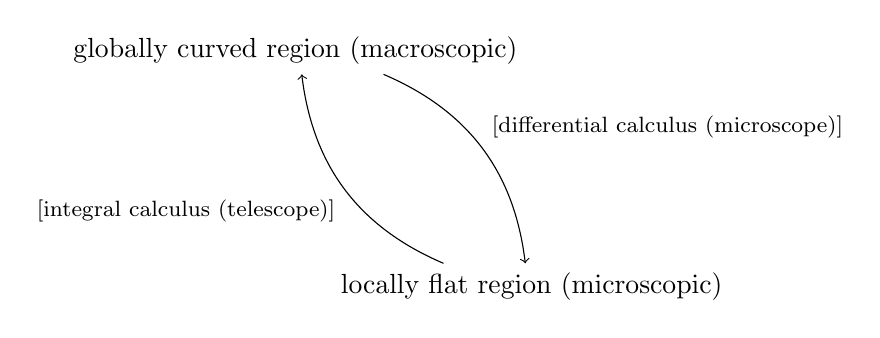
\begin{tikzpicture}[node distance=3cm, auto]
    \node (A) {globally curved region (macroscopic)};
    \node (B) [right of=A] {};
    \node (C) [below of=B] {locally flat region (microscopic)};
    \draw[->, bend left] (A) to node {{\footnotesize  [differential calculus (microscope)]}} (C);
    \draw[->, bend left]  (C) to node {{\footnotesize [integral calculus (telescope)]}} (A);
  \end{tikzpicture}
  %
  \caption{Mappings between globally curved geometry to locally flat geometry. Going from a globally curved region (manifold) to a locally flat region is done using differential calculus, as though using a microscope. On the other hand, going from the flat region to the curved one is done via integral calculus, as though using a telescope.}
  \label{fig:globaltolocaltoglobal}
\end{figure}


\subsubsection{Surface integration}
%
Next, suppose that we want to integrate over a three-dimensional volume at fixed time. We can \emph{generalize} this by asking for the three-dimensional proper \scare{hypersurface} element normal to any given vector ($\tbvec t$ in the case of a spatial volume element at fixed $t$). What does it mean for a vector to be normal to a hypersurface in a curved manifold? The meaning is practically the same as in Euclidean geometry except that the normal is a covector $\cov n$ rather than a vector. The hypersurface is spanned by a set of vectors $\vec t$, called the \lingo{tangent vectors}, orthogonal at $\point P$ to the normal $\cov n$; \ie, $\sprod{\cov n}{\vec t} = 0$. The corresponding normal \emph{vector} $\vec n$ (such that $\vec n\iprod\vec t = 0$) is obtained using the inverse metric, \cref{eq:inversemetricasmap}.

\theme{Hypersurface element.} To find the proper hypersurface element, consider the simpler case of a two-dimensional surface in three-dimensional Euclidean space. The surface area element is written $d\vec s = \uvec n da$, where $\uvec n$ is a unit vector and $da = \tvolel 2$ (the product of two orthonormal coordinate differentials) is the area normal to $\uvec n$. We may expect a similar expression in a general spacetime with $\uvec n$ replaced by the normal covector $\cov n$ and $\tvolel 2$ replaced by $\tvolel 3$. However, the determinant of the metric must appear also. To see how, let us choose our coordinates so that $\tvec n0 = \br{\pm\vec n\iprod\vec n}^{1/2}$ (with a minus sign if $\vec n$ is timelike) and $\tvec n0$ for $i = 1,2,3$. (It is a simple exercise to show that this is always possible provided that $\vec n$ is not a null vector.) In these coordinates, $\tmetric 00 = \pm 1$ and $\tmetric 0i = 0$ for $i = 1,2,3$. We will assume nothing about $\tmetric ij$, the components of the metric in the hypersurface normal to $\cov n$. We know therefore from analogy with \cref{eq:propervolumedifferentialfrommetric} that to get the proper hypersurface area we must multiply the coordinate hypersurface area by $\br{\abs\metric^{(3)}}^{1/3}$, where $\metric^{(3)}$ is the determinant of $\tmetric ij$. But, our four-by-four metric is block diagonal $\br{\tmetric 0i = \tmetric i0 = 0}$, so that the full determinant is $\metric = \tmetric 00\metric^{(3)} = \pm\metric^{(3)}$. (If $\vec n$ is timelike, then $\metric^{(3)} > 0$ and the minus sign is taken; if $\vec n$ is spacelike, then $\metric^{(3)} < 0$ and the plus sign is taken. In either case, in a four-dimensional spacetime, $\metric < 0$.) We can therefore write the proper hypersurface element as
%
\begin{equation}\label{eq:properhypersurfaceelement}
  d\cov\area = \cov n\br{\abs\metric^{(3)}}^{1/2}
             = \cov n\sqrt{-\metric}\,\tvolel 3\,.
\end{equation}
%
This is the desired result.


\subsubsection{Gauss's law}
%
\theme{Vector divergence.} To derive Gauss's law, we first obtain a general expression for the \lingo{divergence of a vector field}. From \cref{eq:componentsofthegradientofavector},
%
\begin{equation}\label{eq:contractionofgradientofvector}
  \tgradcov\mu\tvec v\mu = \ipd\mu\tvec v\mu + \tchris\lambda\lambda\mu\tvec v\mu\,.
\end{equation}

\theme{Comment.} I think it was untold that the divergence is obtained by contracting the gradient, $\div\vec v = \cont\gradcov\vec v$.

From \cref{eq:christoffelsymbolsasfunctionsofmetric}, we get $\tchris\lambda\lambda\mu = \br{1/2}\tinvmet\lambda\kappa\,\ipd\mu\tmetric\lambda\kappa$. Starting from the definition of the determinant in terms of minors and cofactors, one can shaw that the logarithmic derivative of the determinant of $\metric$ is $\ipd\mu\log\metric = \tinvmet\lambda\kappa\ipd\mu\tmetric\lambda\kappa$, where $\log$ is the natural logarithm. Combining these results with \cref{eq:contractionofgradientofvector} gives us an alternative form for the divergence of a vector field:
%
\begin{equation}\label{eq:divergenceofavector}
  \div\vec v = \cont\gradcov\vec v
             = \tgradcov\mu\tvec v\mu
             = \dfrac{1}{\sqrt{-\metric}}\ipd\mu\br{\sqrt{-\metric}\tvec v\mu}\,.
\end{equation}

\theme{Verify.} It is easy to verify that this gives the expected results in polar coordinates, taking care to recall that that standard formulae assume vector components in an orthonormal basis rather than a coordinate basis.

\theme{Example.} Calculate the divergence of a vector $\vec v\in\nespace 3$ defined as
%
\begin{equation*}
  \vec v = \cxpos\sin\cypos\,\uvec\cxpos - \cxpos\cos\cypos\,\uvec\cypos\,.
\end{equation*}
%
\theme{Solution.} First, note that $\vec v$ is expanded on unit basis vectors; the vector is written in its physical form. Thus, express it on coordinate basis, remembering that, for polar coordinates, $\sqrt{\tmetric\cxpos\cxpos} = 1$ and $\sqrt{\tmetric\cypos\cypos} = \cxpos$:
%
\begin{equation*}
  \vec v = \cxpos\sin\cypos\,\tbvec\cxpos - \cos\cypos\,\tbvec\cypos\,.
\end{equation*}
%
Then, find its divergence using \cref{eq:divergenceofavector} and $\sqrt{-\metric} = \cxpos$:
%
\begin{align*}
  \div\vec v &= \dfrac{1}{\sqrt{-\metric}}\ipd\mu\br{\sqrt{-\metric}\tvec v\mu}\,, \\
             &= \dfrac{1}{\cxpos}\br{\ipd\cxpos\cxpos^2\sin\cypos - \ipd\cypos\cxpos\cos\cypos}\,, \\
             &= \dfrac{1}{\cxpos}\br{2\cxpos\sin\cypos + \cxpos\sin\cypos} \,,\\
             &= 3\sin\cypos\,,
\end{align*}
%
which yields the answer.

On the other hand, the problem can be solved by \brand{Mathematica}:
%
\begin{lstlisting}
  Div[{r Sin[\[Theta]], -r Cos[\[Theta]]}, {r, \[Theta]}, "Polar"]
\end{lstlisting}
%
The response is $3\sin\cypos$, agreeing with our solution.

\theme{Technicalities.} Note that \brand{Mathematica} finds $\div\vec v$ for $\vec v$ written on unit basis vectors (physical basis), but it does use polar coordinates -- no coordinate transformation required.

\theme{Gauss's law.} From \cref{eq:divergenceofavector}, we obtain the general form of Gauss's law by integrating over proper volume, \cref{eq:propervolumedifferentialfrommetric}.:
%
\begin{equation}\label{eq:integralformgausslaw}
  \int\div\vec v\,d\vol = \int\tgradcov\mu \tvec v\mu\,d\vol 
                        = \int\ipd\mu\br{\sqrt{-\metric}\,\tvec v\mu}\,\tvolel 4
                        = \oint\tvec v\mu\tcov n\nu\sqrt{-\metric}\,\tvolel 3\,.
\end{equation}
%
\theme{Interpretation.} The four-dimensional integral is a \lingo{total derivative}, allowing it to be reduced to a three-dimensional integral over the closed hypersurface with normal covector $\cov n = \tcov n\mu\tbcov\mu$ bounding the four-volume region of integration (\eg, $\cov n = \tbcov t$ if we compute the difference of three-volume integrals at two times). Although it is difficult to visualize a four-volume or a closed three-dimensional hypersurface, the meaning is the same as for the standard Gauss's law in space three dimensions except that one more dimension has been added.
%
\begin{quotation}
  It is important to note that \cref{eq:integralformgausslaw} is valid for any coordinate system.
\end{quotation}


\subsection{Parallel transport and geodesics}

\subsubsection{Differentiation along a curve}
%
\theme{Differentiation along a curve.} As a prelude to parallel transport, consider another form of differentiation: \lingo{differentiation along a curve}. A \lingo{curve} is a parametrized path trough spacetime: $\curve\vat\ptime$, where $\ptime$ is a parameter that varies smoothly and monotonically along the path.

\theme{Lingo.} There are subtle differences between a \lingo{curve}, a \lingo{trajectory}, an \lingo{orbit}, and a \lingo{world line}. A curve is a parametrized path. A trajectory is also a curve. But an orbit is a closed curve and a world line is a curve in relativity -- it includes the time dimension. Sometimes \lingo{history} is used as wold line.

The curve has a tangent vector $\vec v\defas d_\ptime\vec\pos = d\vec\pos/d\ptime = d_\ptime\tvec\pos\mu\,\tbvec\mu$. If we wish, then we could make $\vec v$ a unit vector, provided $\vec v$ is not null, by setting $d\ptime = \br{\pm d\vec\pos\iprod d\vec\pos}^{1/2}$ to measure path length along the curve (with a minus sign if $d\vec\pos$ is timelike). However, we will impose no such a restriction in general. Now, suppose that we have a scalar field $f$ defined along the curve (if not all of spacetime). We define the derivative along the curve by a simple extension of \cref{eq:definitionofgradient,eq:coordinatefreegradient}:
%
\begin{equation}\label{eq:derivativealongacurve}
  d_\ptime f = \dfrac{df}{d\ptime}
             \defas \cgradcov{\vec v} f
             \defas \sprod{\gradcov f}{\vec v}
             = \tvec v\mu\ipd\mu f\,,\quad
  \vec v = d_\ptime\vec\pos
         = \dfrac{d\vec\pos}{d\ptime}\,.
\end{equation}

\theme{Symbol.} We have introduced the symbol $\cgradcov{\vec v}$ for the covariant derivative along $\vec v$, the tangent vector to the curve $\curve\vat\ptime$. 
%
\begin{quotation}
  This is a natural generalization of $\tgradcov\mu$, the covariant derivative along the basis vector $\tbvec\mu$.
\end{quotation}

For the derivative of a scalar field, $\cgradcov{\vec v}$ involves just the partial derivatives $\ipd\mu$. Suppose, however, that we differentiate a vector field $\vec a$ along the curve. Now, the components of the gradient $\tgradcov\mu\tvec a\nu$ are \emph{not} simply the partial derivatives. As we saw earlier, the covariant derivative of a vector field differs from the partial derivatives. The same is true when we project the gradient onto the tangent vector $\vec v$ along a curve:
%
\begin{equation}\label{eq:gradientprojectionalongacurve}
  d_\ptime\vec a \defas D_\ptime\tvec a\mu\tbvec\mu
                 \defas \dfrac{D\tvec a\mu}{D\ptime}\tbvec\mu
                 \defas \cgradcov{\vec v}\vec a
                 \defas \sprod{\gradcov\vec a}{\vec v}
                 = \tvec v\kappa\br{\tgradcov\kappa\tvec a\mu}\tbvec\mu
                 = \br{d_\ptime\tvec a\mu + \tchris\mu\kappa\lambda\tvec v\kappa\tvec a\lambda}\tbvec\mu\,.
\end{equation}
%
We retain the symbol $\cgradcov{\vec v}$ to indicate the covariant derivative along $\vec v$, but we have introduced the new notation
%
\begin{equation*}
  D_\ptime = \dfrac{D}{D\ptime} = \tvec v\mu\tgradcov\mu
           \neq d_\ptime = \dfrac{d}{d\ptime} = \tvec v\mu\ipd\mu\,.
\end{equation*}


\subsubsection{Parallel transport}
%
\theme{Definition.} The derivative of a vector along a curve leads us to an important concept called \lingo{parallel transport}. Suppose we have a curve $\curve\vat\ptime$ with tangent $\vec v$ and a vector $\vec a\vat 0$ define at one point on the curve (call it $\ptime = 0$). We define a procedure called parallel transport by defining a vector $\vec a\vat\ptime$ along each point of the curve in such a way that $D_\ptime\tvec a\mu = 0$:
%
\begin{equation}\label{eq:paralleltransport}
  \cgradcov{\vec v}\vec a = 0\qquad\iff\qquad\text{parallel transport of $\vec a$ along $\vec v$}\,.
\end{equation}
%
Over a small distance interval, this procedure is equivalent to transporting the vector $\vec a$ along the curve in such a way that the vector remains parallel to itself with constant length:
%
\begin{equation*}
  \vec a\vat{\ptime + \Delta\ptime} = \vec a\vat\ptime + O\vat{\Delta\ptime}^2\,.
\end{equation*}
%
In a locally flat coordinate system, with Christoffel's symbols vanishing at $\curve\vat\ptime$, the components of the vector do not change as the vector is transported along the curve. If the space were globally flat, then the components would not change at all no matter how the vector is transported. This is not the case in a curved space or in a flat space with curvilinear coordinates.
%
\begin{figure}[bt]
  \capstart
  \centering
  %
  \includegraphics[width=0.70\textwidth]{./graph/parallel-transport-1}
  %
  \caption{Parallel transport in curved space. The vector is kept parallel to itself and tangent to the curve.}
  \label{fig:paralleltransport}
\end{figure}


\subsubsection{Geodesics}
%
\theme{Definition.} Parallel transport can be used to define a special class of curves called \lingo{geodesics}. A geodesic curve is one that parallel-transports its own tangent vector $\vec v = d_\ptime\vec\pos$; \ie, a curve that satisfies
%
\begin{equation*}
  \cgradcov{\vec v}\vec v = 0\,.
\end{equation*}
%
In other words, not only is $\vec v$ kept parallel to itself (with constant magnitude) along the curve, the curve continues to point in the same direction all along the path. A geodesic is the natural extension of the definition of \scare{straight line} to a curved manifold. Using \cref{eq:gradientprojectionalongacurve,eq:paralleltransport}, we get a second-order differential equation for the coordinates of a geodesic curve:
%
\begin{equation}\label{eq:coordinatesofageodesic}
  D_\ptime\tvec v\mu = d_\ptime\tvec v\mu + \tchris\mu\kappa\lambda\tvec v\kappa\tvec v\lambda = 0
    \qquad\text{for a geodesic,}\qquad
  \tvec v\mu \defas d_\ptime\tvec\pos\mu\,.
\end{equation}
%
\theme{Verify correspondence.} Indeed, in locally flat coordinates (such that Christoffel's symbols vanish at a point), this is the equation of a straight line. However, in a curved space Christoffel's symbols cannot be made to vanish everywhere. A well-known example of a geodesic in a curved space is a great circle on a sphere, \cref{fig:greatcirclesonsphere}.
%
%
\begin{figure}[bt]
  \capstart
  \centering
  %
  \includegraphics[width=0.70\textwidth]{./graph/great-circles-sphere}
  %
  \caption{Great circle on a sphere, an example of a geodesic}
  \label{fig:greatcirclesonsphere}
\end{figure}

\theme{Technicalities.} There are several technical points worth noting about geodesic curves. 
%
\begin{enumerate}
  \item $\vec v\iprod\vec v = \metric\vat{\vec v,\vec v}$ is constant along a geodesic because $d_\ptime\vec v = 0$ and $\cgradcov{\vec v}\metric = 0$. Therefore, a geodesic may be classified by its tangent vector as being either timelike ($\vec v\iprod\vec v < 0$), spacelike ($\vec v\iprod\vec v > 0$), or null ($\vec v\iprod\vec v = 0$). 
  \item a nonlinear transformation of the parameter $\ptime$ will invalidate \cref{eq:coordinatesofageodesic}. In other words, if $\tvec\pos\mu\vat\ptime$ solves \cref{eq:coordinatesofageodesic}, then $\tcov y\mu\vat\ptime\defas\tvec\pos\mu\vat{\xi\vat\ptime}$ will not solve it unless $\xi = a\ptime + b$, for some constants $a,b$. Only a special class of parameters, called \lingo{affine parameters}, can parametrize geodesic curves.
\end{enumerate}
%
\theme{Affine parameter takes care of itself.} The affine parameter has a special interpretation for a non-null geodesic. We deduce this relation from the constancy along the geodesic of $\vec v\iprod\vec v = \br{d\vec\pos\iprod d\vec\pos/\br{d\ptime^2}}\defas a$, implying $ds = ad\ptime$ and therefore $s = a\ptime + b$, where $s$ is the path length, \cref{eq:squareddistancebetweenevents}. For a non-null geodesic ($\vec v\iprod\vec v\neq 0$), all affine parameters are linear functions of path length. The linear scaling of path length amounts simply to the freedom to change units of length and to choose any point as $\ptime = 0$. Note that originally we imposed no constraints on the parameter but that, for a non-null geodesic, the parameter naturally turns out to measure path length. In fact, we don't need to worry about the parameter in any case, because it will take care of itself (even for a null geodesic), when \cref{eq:coordinatesofageodesic} is integrated. One can always reparametrize the solution later or eliminate the parameter altogether by replacing it with one of the coordinates along the geodesic.

\theme{Geodesic from stationary action.} Another interesting point is that the total path length is stationary for a geodesic:
%
\begin{equation}\label{eq:geodesicisstationary}
  \delta\int_{\point A}^{\point B}\,ds 
    = \delta\int_{\point A}^{\point B}
        \br{\pm\tmetric\mu\nu\,d_\ptime\tvec\pos\mu d_\ptime\tvec\pos\nu}^{1/2}\,d\ptime = 0\,.
\end{equation}
%
The $\delta$ refers to a variation of the integral arising from a variation of the curve, $\curve\vat\ptime\mapsto\tvec\pos\mu\vat\ptime + \delta\tvec\pos\mu\vat\ptime$, with fixed endpoints. The metric components are considered here to be functions of the coordinates. We leave it as an exercise for the reader to show that \cref{eq:geodesicisstationary} leads to \cref{eq:coordinatesofageodesic}. \Cref{eq:geodesicisstationary} is a curved space generalization of the statement that a straight line is the shortest path between two points in flat space.


\subsubsection{Integrals of motion and Killing vectors}
%
\begin{equation}
  \eqtxt{missing}
\end{equation}
%
\begin{equation}
  \eqtxt{missing}
\end{equation}
%
\begin{equation}
  \eqtxt{missing}
\end{equation}


\subsection{Curvature}
%
\theme{Intro.} We introduce curvature by considering parallel transport around a general (non-geodesic) closed curve.
%
\begin{quotation}
  In a nonflat space, this procedure can lead to a different vector at the end of the curve than the one at the beginning.
\end{quotation}
%
Consider, for instance, a sphere. Suppose we have a vector pointing east on the equation at longitude \ang{0}. We parallel transport the vector eastward on the equator by \ang{180}. At each point on the equator, the vector points east. Now the vector is parallel transported along a line of constant longitude over the pole and back to the starting point. At each point on this second part of the curve, the vector points at right angles to the curve, and its direction never changes. Yet, at the end of the curve, at the same point where the curve started, the vector points west!

This result also implies that parallel transport along two different curves may lead to different final vectors. If a vector on the equator is parallel-transported to the opposite side of a sphere along the equator, and, alternatively, over the pole (in fact, both of these curves are geodesics), the resulting vectors will point in opposite directions. This recalls our earlier point that 
%
\begin{quotation}
  it is not possible to directly compare vectors defined at different points in a curved manifold.
\end{quotation}

\theme{Riemann tensor.} A change in the vector $\vec a$ as a result of parallel transport over a closed curve is a dead giveaway of spatial curvature. Suppose that our curve consists of four infinitesimal segments: $d\vec\pos_1, d\vec\pos_2$, and $-d\vec\pos_1,-d\vec\pos_2$. In a flat space this would be called a parallelogram and the difference $d\vec a$ between the final and initial vectors would vanish. In a curved space, the change is a linear function of $\vec a,d\vec\pos_1,d\vec\pos_2$:
%
\begin{equation}\label{eq:definitionofriemannstensor}
  d\vec a\vat{\cslot} \defas \riemann\vat{\cslot,\vec a,d\vec\pos_1,d\vec\pos_2}
                      = \tbvec\mu\triemann\mu\nu\kappa\lambda\tvec a\nu\,d\tvec\pos\kappa d\tvec\pos\lambda\,.
\end{equation}
%
We have defined a rank $\torder 13$ tensor called \lingo{Riemann's curvature tensor}. It is relatively straightforward exercise to determine the components of Riemann's tensor using \cref{eq:gradientprojectionalongacurve,eq:paralleltransport}. The result is
%
\begin{equation}\label{eq:componentsofriemannstensor}
  \triemann\mu\nu\kappa\lambda = \ipd\kappa\tchris\mu\nu\lambda 
                               - \ipd\lambda\tchris\mu\nu\kappa
                               + \tchris\mu\alpha\kappa \tchris\alpha\nu\lambda
                               - \tchris\mu\alpha\lambda \tchris\alpha\nu\kappa \,.
\end{equation}
%
Note that some authors define the components with opposite sign. Our sign convention follows MTW, Wald, and Schutz.

\theme{Riemann's tensor uniqueness.} Note that Riemann's tensor involves the first and second partial derivatives of the metric (through Christoffel's symbols). Riemann's tensor is the only tensor that can be constructed from the metric tensor and its first and second partial derivatives and is linear in the second derivatives. Recall that one can always define locally flat coordinates such that $\tchris\mu\nu\lambda = 0$, everywhere unless the space is \emph{globally flat}.
%
\begin{quotation}
  Riemann's tensor vanishes everywhere if and only if the manifold is globally flat.
\end{quotation}

\theme{Riemann from metric.} An alternative derivation of Riemann's tensor is based on the non-commutativity of the second covariant derivatives of a vector. The covariant derivative $\tgradcov\mu\tvec a\nu$ is defined in \cref{eq:componentsofthegradientofavector}; as an order $\torder 11$ tensor, this quantity has a covariant derivative defined as in \cref{eq:gradientidtensor}. It can be shown that:
%
\begin{equation}\label{eq:riemanntensorequality}
  \br{\tgradcov\kappa\tgradcov\lambda - \tgradcov\lambda\tgradcov\kappa}\tvec v\mu 
    = \triemann\mu\nu\kappa\lambda\tvec v\nu\,.
\end{equation}
%
with Riemann's tensor components defined as in \cref{eq:componentsofriemannstensor}.

\theme{Symmetries.} If we lower an index on Riemann's tensor components, then we get the components of a $\torder 40$ tensor:
%
\begin{equation}\label{eq:lowerindicesinriemanntensor}
  \tensor{\riemann}{_\mu_\nu_\kappa_\lambda} = \tmetric\mu\alpha\triemann\alpha\nu\kappa\lambda
    = \dfrac 12
      \br{
        \tensor{\metric}{_\mu_\lambda_,_\nu_\kappa} - \tensor{\metric}{_\mu_\kappa_,_\nu_\lambda}
        + \tensor{\metric}{_\nu_\kappa_,_\mu_\lambda} - \tensor{\metric}{_\nu_\lambda_,_\mu_\kappa}
      }
      + \tmetric\alpha\beta
      \br{
        \tchris\alpha\mu\lambda \tchris\beta\nu\kappa - \tchris\alpha\mu\kappa \tchris\beta\nu\lambda
      }\,,
\end{equation}
%
where we have used commas to denote partial derivatives for notational convenience. In this form, it is easy to determine the following symmetry properties of Riemann's tensor:
%
\begin{equation}\label{eq:riemanntensorsymmetryproperties}
  \tensor{\riemann}{_\mu_\nu_\kappa_\lambda} 
    = \tensor{\riemann}{_\kappa_\lambda_\mu_\nu}
    = -\tensor{\riemann}{_\nu_\mu_\kappa_\lambda}
    = -\tensor{\riemann}{_\mu_\nu_\lambda_\kappa}\,,
  \qquad
  \tensor{\riemann}{_\mu_\nu_\kappa_\lambda}
  + \tensor{\riemann}{_\mu_\kappa_\lambda_\nu}
  + \tensor{\riemann}{_\mu_\lambda_\nu_\kappa}
  = 0\,.
\end{equation}
%
It can be shown that these symmetries reduce the number of independent components of Riemann's tensor from $4^4$ to $20$.


\subsubsection{Bianchi identities, Ricci tensor, and Einstein tensor}
%
\theme{Bianchi.} By differentiating the components of Riemann's tensor, one can prove \lingo{Bianchi's identities}:
%
\begin{equation}\label{eq:bianchiidentities}
  \tgradcov\sigma\triemann\mu\nu\kappa\lambda 
  + \tgradcov\kappa\triemann\mu\nu\lambda\sigma 
  + \tgradcov\lambda\triemann\mu\nu\sigma\kappa
  = 0\,.
\end{equation}
%
\theme{Ricci tensor.} Note that the gradient symbols denote the covariant derivatives and \emph{not} the partial derivatives (otherwise, we would not have a tensor equation). Bianchi's identities imply the vanishing of the divergence of a certain $\torder 20$ tensor. We first define a symmetric contraction of Riemann's tensor, known as \lingo{Ricci's tensor}:
%
\begin{equation}\label{eq:riccitensordefinition}
  \ricci\vat{\vslot,\vslot} 
    = \cont_{1,3}\riemann\vat{\cslot,\vslot,\vslot,\vslot}
    = \tricci\mu\nu \defas \triemann\alpha\mu\alpha\nu
    = \tricci\nu\mu
    = \ipd\kappa\tchris\kappa\mu\nu - \ipd\mu\tchris\kappa\kappa\nu 
      + \tchris\kappa\kappa\lambda\tchris\lambda\mu\nu
      - \tchris\kappa\mu\lambda\tchris\lambda\kappa\nu\,.
\end{equation}
%
\theme{Ricci scalar.} One can shaw from \cref{eq:riemanntensorsymmetryproperties} that any other contraction of Riemann's tensor either vanishes or is proportional to Ricci's tensor. The contraction of Ricci's tensor is called \lingo{Ricci's scalar}:
%
\begin{equation}\label{eq:ricciscalardefinition}
  \sricci \defas \cont\ricci\vat{\vslot,\vslot}
    = \invmet\vat{\ricci\vat{\vslot,\vslot}}
    = \tinvmet\mu\nu\tricci\mu\nu\,.
\end{equation}
%
\theme{Einstein tensor.} Contracting Bianchi's identities twice and using the antisymmetry of Riemann's tensor, one obtains the following relation:
%
\begin{equation}\label{eq:einsteinstensordefinition}
  \gradcov\einstein = 0\implies
  \tgradcov\nu\teinstein\mu\nu = 0\,,\qquad
  \teinstein\mu\nu \defas \tricci\mu\nu - \dfrac 12\tmetric\mu\nu\sricci = \teinstein\nu\mu\,.
\end{equation}
%
The symmetric tensor $\teinstein\mu\nu$ that we have introduced is called \lingo{Einstein's tensor}. \Cref{eq:einsteinstensordefinition} is a math identity, \emph{not} a physics law. However., it illustrates a deep connection between math symmetries and physical conservation laws.

Misner style:
%
\begin{align*}
  \mricci\vat{\vslot,\vslot} &= \cont_{1,3}\mriemann\vat{\cslot,\vslot,\vslot,\vslot}\,,\quad \\
  \sricci &= \mmetric\vat{\mricci\vat{\vslot,\vslot}}\,,\quad \\
  \gradcov\meinstein &= 0\,,\\
  \gradcov\meinstein\vat{\cslot,\cslot} &= \mricci\vat{\cslot,\cslot}
    - \dfrac 12\sricci\minvmet\vat{\cslot,\cslot}\,.
\end{align*}
